\documentclass[twoside]{book}

% Packages required by doxygen
\usepackage{fixltx2e}
\usepackage{calc}
\usepackage{doxygen}
\usepackage[export]{adjustbox} % also loads graphicx
\usepackage{graphicx}
\usepackage[utf8]{inputenc}
\usepackage{makeidx}
\usepackage{multicol}
\usepackage{multirow}
\PassOptionsToPackage{warn}{textcomp}
\usepackage{textcomp}
\usepackage[nointegrals]{wasysym}
\usepackage[table]{xcolor}

% Font selection
\usepackage[T1]{fontenc}
\usepackage[scaled=.90]{helvet}
\usepackage{courier}
\usepackage{amssymb}
\usepackage{sectsty}
\renewcommand{\familydefault}{\sfdefault}
\allsectionsfont{%
  \fontseries{bc}\selectfont%
  \color{darkgray}%
}
\renewcommand{\DoxyLabelFont}{%
  \fontseries{bc}\selectfont%
  \color{darkgray}%
}
\newcommand{\+}{\discretionary{\mbox{\scriptsize$\hookleftarrow$}}{}{}}

% Page & text layout
\usepackage{geometry}
\geometry{%
  a4paper,%
  top=2.5cm,%
  bottom=2.5cm,%
  left=2.5cm,%
  right=2.5cm%
}
\tolerance=750
\hfuzz=15pt
\hbadness=750
\setlength{\emergencystretch}{15pt}
\setlength{\parindent}{0cm}
\setlength{\parskip}{3ex plus 2ex minus 2ex}
\makeatletter
\renewcommand{\paragraph}{%
  \@startsection{paragraph}{4}{0ex}{-1.0ex}{1.0ex}{%
    \normalfont\normalsize\bfseries\SS@parafont%
  }%
}
\renewcommand{\subparagraph}{%
  \@startsection{subparagraph}{5}{0ex}{-1.0ex}{1.0ex}{%
    \normalfont\normalsize\bfseries\SS@subparafont%
  }%
}
\makeatother

% Headers & footers
\usepackage{fancyhdr}
\pagestyle{fancyplain}
\fancyhead[LE]{\fancyplain{}{\bfseries\thepage}}
\fancyhead[CE]{\fancyplain{}{}}
\fancyhead[RE]{\fancyplain{}{\bfseries\leftmark}}
\fancyhead[LO]{\fancyplain{}{\bfseries\rightmark}}
\fancyhead[CO]{\fancyplain{}{}}
\fancyhead[RO]{\fancyplain{}{\bfseries\thepage}}
\fancyfoot[LE]{\fancyplain{}{}}
\fancyfoot[CE]{\fancyplain{}{}}
\fancyfoot[RE]{\fancyplain{}{\bfseries\scriptsize Generated by Doxygen }}
\fancyfoot[LO]{\fancyplain{}{\bfseries\scriptsize Generated by Doxygen }}
\fancyfoot[CO]{\fancyplain{}{}}
\fancyfoot[RO]{\fancyplain{}{}}
\renewcommand{\footrulewidth}{0.4pt}
\renewcommand{\chaptermark}[1]{%
  \markboth{#1}{}%
}
\renewcommand{\sectionmark}[1]{%
  \markright{\thesection\ #1}%
}

% Indices & bibliography
\usepackage{natbib}
\usepackage[titles]{tocloft}
\setcounter{tocdepth}{3}
\setcounter{secnumdepth}{5}
\makeindex

% Hyperlinks (required, but should be loaded last)
\usepackage{ifpdf}
\ifpdf
  \usepackage[pdftex,pagebackref=true]{hyperref}
\else
  \usepackage[ps2pdf,pagebackref=true]{hyperref}
\fi
\hypersetup{%
  colorlinks=true,%
  linkcolor=blue,%
  citecolor=blue,%
  unicode%
}

% Custom commands
\newcommand{\clearemptydoublepage}{%
  \newpage{\pagestyle{empty}\cleardoublepage}%
}

\usepackage{caption}
\captionsetup{labelsep=space,justification=centering,font={bf},singlelinecheck=off,skip=4pt,position=top}

%===== C O N T E N T S =====

\begin{document}

% Titlepage & ToC
\hypersetup{pageanchor=false,
             bookmarksnumbered=true,
             pdfencoding=unicode
            }
\pagenumbering{roman}
\begin{titlepage}
\vspace*{7cm}
\begin{center}%
{\Large My Project }\\
\vspace*{1cm}
{\large Generated by Doxygen 1.8.11}\\
\end{center}
\end{titlepage}
\clearemptydoublepage
\tableofcontents
\clearemptydoublepage
\pagenumbering{arabic}
\hypersetup{pageanchor=true}

%--- Begin generated contents ---
\chapter{Hierarchical Index}
\section{Class Hierarchy}
This inheritance list is sorted roughly, but not completely, alphabetically\+:\begin{DoxyCompactList}
\item \contentsline{section}{Steering\+Control}{\pageref{classSteeringControl}}{}
\item \contentsline{section}{Steering\+Control\+Output}{\pageref{classSteeringControlOutput}}{}
\item \contentsline{section}{virtual\+Point}{\pageref{classvirtualPoint}}{}
\begin{DoxyCompactList}
\item \contentsline{section}{Mock\+Point}{\pageref{classMockPoint}}{}
\item \contentsline{section}{Point}{\pageref{classPoint}}{}
\end{DoxyCompactList}
\end{DoxyCompactList}

\chapter{Class Index}
\section{Class List}
Here are the classes, structs, unions and interfaces with brief descriptions\+:\begin{DoxyCompactList}
\item\contentsline{section}{\hyperlink{classMockPoint}{Mock\+Point} }{\pageref{classMockPoint}}{}
\item\contentsline{section}{\hyperlink{classPoint}{Point} \\*Class \hyperlink{classPoint}{Point} is declared with its two data members namely X and Y and four methods \+: get\+\_\+x set\+\_\+x get\+\_\+y set\+\_\+y }{\pageref{classPoint}}{}
\item\contentsline{section}{\hyperlink{classSteeringControl}{Steering\+Control} \\*Class \hyperlink{classSteeringControl}{Steering\+Control} is declared with its four double type private data members (wheelbase, trackwidth, cgz, vehicle\+Velocity) and four \hyperlink{classPoint}{Point(class)}type data members (Target, Veh\+Front, Veh\+Right, Veh\+Left) class \hyperlink{classSteeringControl}{Steering\+Control} has seven methods \+: compute\+\_\+and\+\_\+update\+\_\+coordinate set\+\_\+target\+\_\+and\+\_\+veh\+\_\+velocity get\+\_\+distance has\+\_\+reached\+\_\+target, get\+\_\+front\+\_\+coordinate, get\+\_\+left\+\_\+coordinate, get\+\_\+right\+\_\+coordinate }{\pageref{classSteeringControl}}{}
\item\contentsline{section}{\hyperlink{classSteeringControlOutput}{Steering\+Control\+Output} \\*Class \hyperlink{classSteeringControlOutput}{Steering\+Control\+Output} is declared with its three data members namely Left\+Wheel\+Speed, Right\+Wheel\+Speed and Steering\+Angle and have six methods \+: get\+\_\+left\+\_\+wheel\+\_\+speed set\+\_\+left\+\_\+wheel\+\_\+speed get\+\_\+right\+\_\+wheel\+\_\+speed set\+\_\+right\+\_\+wheel\+\_\+speed get\+\_\+steering\+\_\+angle set\+\_\+steering\+\_\+angle }{\pageref{classSteeringControlOutput}}{}
\item\contentsline{section}{\hyperlink{classvirtualPoint}{virtual\+Point} }{\pageref{classvirtualPoint}}{}
\end{DoxyCompactList}

\chapter{File Index}
\section{File List}
Here is a list of all files with brief descriptions\+:\begin{DoxyCompactList}
\item\contentsline{section}{/home/saurav/\+Documents/\+Steering Control Module/cpp-\/boilerplate/app/\hyperlink{app_2main_8cpp}{main.\+cpp} \\*Takes target coordinate and vehicle velocity as input and provides individual wheel speed and steering angle as output until the vehicle has reached the defined target coordinate }{\pageref{app_2main_8cpp}}{}
\item\contentsline{section}{/home/saurav/\+Documents/\+Steering Control Module/cpp-\/boilerplate/app/\hyperlink{Point_8cpp}{Point.\+cpp} }{\pageref{Point_8cpp}}{}
\item\contentsline{section}{/home/saurav/\+Documents/\+Steering Control Module/cpp-\/boilerplate/app/\hyperlink{SteeringControl_8cpp}{Steering\+Control.\+cpp} \\*Takes target coordinate and vehicle velocity as input and provides individual wheel speed, steering angle, new coordinates of the vehicle wheel endafter a dt time ,such that the vehicle movement shall be toward the target point.\+The standard time latency is considered to be 0.\+01 sec }{\pageref{SteeringControl_8cpp}}{}
\item\contentsline{section}{/home/saurav/\+Documents/\+Steering Control Module/cpp-\/boilerplate/app/\hyperlink{SteeringControlOutput_8cpp}{Steering\+Control\+Output.\+cpp} }{\pageref{SteeringControlOutput_8cpp}}{}
\item\contentsline{section}{/home/saurav/\+Documents/\+Steering Control Module/cpp-\/boilerplate/demo/\hyperlink{demo_2main_8cpp}{main.\+cpp} \\*Takes target coordinate and vehicle velocity as input and provides individual wheel speed and steering angle as output untill the vehicle has reached the defined target coordinate. It also prints the and speed of individual drive wheels,steering angle in degree and the coorinates of wheel ends }{\pageref{demo_2main_8cpp}}{}
\item\contentsline{section}{/home/saurav/\+Documents/\+Steering Control Module/cpp-\/boilerplate/include/\hyperlink{Point_8h}{Point.\+h} }{\pageref{Point_8h}}{}
\item\contentsline{section}{/home/saurav/\+Documents/\+Steering Control Module/cpp-\/boilerplate/include/\hyperlink{SteeringControl_8h}{Steering\+Control.\+h} \\*Header file for declaring the class \hyperlink{classSteeringControl}{Steering\+Control},its attributes and its methods along with class \hyperlink{classSteeringControlOutput}{Steering\+Control\+Output}, class \hyperlink{classPoint}{Point} and their data members }{\pageref{SteeringControl_8h}}{}
\item\contentsline{section}{/home/saurav/\+Documents/\+Steering Control Module/cpp-\/boilerplate/include/\hyperlink{SteeringControlOutput_8h}{Steering\+Control\+Output.\+h} }{\pageref{SteeringControlOutput_8h}}{}
\item\contentsline{section}{/home/saurav/\+Documents/\+Steering Control Module/cpp-\/boilerplate/include/\hyperlink{virtualPoint_8h}{virtual\+Point.\+h} }{\pageref{virtualPoint_8h}}{}
\item\contentsline{section}{/home/saurav/\+Documents/\+Steering Control Module/cpp-\/boilerplate/test/\hyperlink{test_2main_8cpp}{main.\+cpp} \\*Runs unit tests using google gtest framework }{\pageref{test_2main_8cpp}}{}
\item\contentsline{section}{/home/saurav/\+Documents/\+Steering Control Module/cpp-\/boilerplate/test/\hyperlink{PointTest_8cpp}{Point\+Test.\+cpp} }{\pageref{PointTest_8cpp}}{}
\item\contentsline{section}{/home/saurav/\+Documents/\+Steering Control Module/cpp-\/boilerplate/test/\hyperlink{SteeringControlOutputTest_8cpp}{Steering\+Control\+Output\+Test.\+cpp} }{\pageref{SteeringControlOutputTest_8cpp}}{}
\item\contentsline{section}{/home/saurav/\+Documents/\+Steering Control Module/cpp-\/boilerplate/test/\hyperlink{SteeringControlTest_8cpp}{Steering\+Control\+Test.\+cpp} }{\pageref{SteeringControlTest_8cpp}}{}
\end{DoxyCompactList}

\chapter{Class Documentation}
\hypertarget{classMockPoint}{}\section{Mock\+Point Class Reference}
\label{classMockPoint}\index{Mock\+Point@{Mock\+Point}}


Inheritance diagram for Mock\+Point\+:
\nopagebreak
\begin{figure}[H]
\begin{center}
\leavevmode
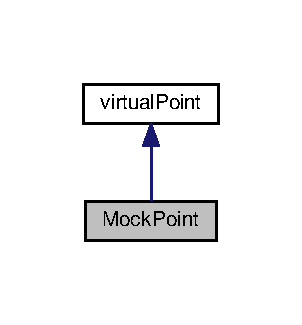
\includegraphics[width=145pt]{classMockPoint__inherit__graph}
\end{center}
\end{figure}


Collaboration diagram for Mock\+Point\+:
\nopagebreak
\begin{figure}[H]
\begin{center}
\leavevmode
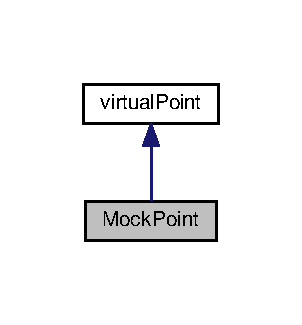
\includegraphics[width=145pt]{classMockPoint__coll__graph}
\end{center}
\end{figure}
\subsection*{Public Member Functions}
\begin{DoxyCompactItemize}
\item 
\hyperlink{classMockPoint_a4b4a7a06cd9dc8421958a65940aac962}{M\+O\+C\+K\+\_\+\+M\+E\+T\+H\+O\+D0} (\hyperlink{classvirtualPoint_afe6be96f2ab063515a78087d9ce22ddf}{get\+\_\+x}, double())
\item 
\hyperlink{classMockPoint_ab9c9f8084a5ff1cd39b6a70a09302a8e}{M\+O\+C\+K\+\_\+\+M\+E\+T\+H\+O\+D1} (\hyperlink{classvirtualPoint_a2e0023f0dffbb82aee6d358a3998807d}{set\+\_\+x}, void(double x\+\_\+coordinate\+\_\+value))
\item 
\hyperlink{classMockPoint_a0e195a76b458d639de4345e40348d8e5}{M\+O\+C\+K\+\_\+\+M\+E\+T\+H\+O\+D0} (\hyperlink{classvirtualPoint_ab7149e207c73c324a5028c160d493ac4}{get\+\_\+y}, double())
\item 
\hyperlink{classMockPoint_aa53d24c9da3b37bbc6d882df0bb19aa9}{M\+O\+C\+K\+\_\+\+M\+E\+T\+H\+O\+D1} (\hyperlink{classvirtualPoint_afbeef257f2fe3581b6f302e085968f79}{set\+\_\+y}, void(double y\+\_\+coordinate\+\_\+value))
\end{DoxyCompactItemize}


\subsection{Member Function Documentation}
\index{Mock\+Point@{Mock\+Point}!M\+O\+C\+K\+\_\+\+M\+E\+T\+H\+O\+D0@{M\+O\+C\+K\+\_\+\+M\+E\+T\+H\+O\+D0}}
\index{M\+O\+C\+K\+\_\+\+M\+E\+T\+H\+O\+D0@{M\+O\+C\+K\+\_\+\+M\+E\+T\+H\+O\+D0}!Mock\+Point@{Mock\+Point}}
\subsubsection[{\texorpdfstring{M\+O\+C\+K\+\_\+\+M\+E\+T\+H\+O\+D0(get\+\_\+x, double())}{MOCK_METHOD0(get_x, double())}}]{\setlength{\rightskip}{0pt plus 5cm}Mock\+Point\+::\+M\+O\+C\+K\+\_\+\+M\+E\+T\+H\+O\+D0 (
\begin{DoxyParamCaption}
\item[{{\bf get\+\_\+x}}]{, }
\item[{double()}]{}
\end{DoxyParamCaption}
)}\hypertarget{classMockPoint_a4b4a7a06cd9dc8421958a65940aac962}{}\label{classMockPoint_a4b4a7a06cd9dc8421958a65940aac962}
\index{Mock\+Point@{Mock\+Point}!M\+O\+C\+K\+\_\+\+M\+E\+T\+H\+O\+D0@{M\+O\+C\+K\+\_\+\+M\+E\+T\+H\+O\+D0}}
\index{M\+O\+C\+K\+\_\+\+M\+E\+T\+H\+O\+D0@{M\+O\+C\+K\+\_\+\+M\+E\+T\+H\+O\+D0}!Mock\+Point@{Mock\+Point}}
\subsubsection[{\texorpdfstring{M\+O\+C\+K\+\_\+\+M\+E\+T\+H\+O\+D0(get\+\_\+y, double())}{MOCK_METHOD0(get_y, double())}}]{\setlength{\rightskip}{0pt plus 5cm}Mock\+Point\+::\+M\+O\+C\+K\+\_\+\+M\+E\+T\+H\+O\+D0 (
\begin{DoxyParamCaption}
\item[{{\bf get\+\_\+y}}]{, }
\item[{double()}]{}
\end{DoxyParamCaption}
)}\hypertarget{classMockPoint_a0e195a76b458d639de4345e40348d8e5}{}\label{classMockPoint_a0e195a76b458d639de4345e40348d8e5}
\index{Mock\+Point@{Mock\+Point}!M\+O\+C\+K\+\_\+\+M\+E\+T\+H\+O\+D1@{M\+O\+C\+K\+\_\+\+M\+E\+T\+H\+O\+D1}}
\index{M\+O\+C\+K\+\_\+\+M\+E\+T\+H\+O\+D1@{M\+O\+C\+K\+\_\+\+M\+E\+T\+H\+O\+D1}!Mock\+Point@{Mock\+Point}}
\subsubsection[{\texorpdfstring{M\+O\+C\+K\+\_\+\+M\+E\+T\+H\+O\+D1(set\+\_\+x, void(double x\+\_\+coordinate\+\_\+value))}{MOCK_METHOD1(set_x, void(double x_coordinate_value))}}]{\setlength{\rightskip}{0pt plus 5cm}Mock\+Point\+::\+M\+O\+C\+K\+\_\+\+M\+E\+T\+H\+O\+D1 (
\begin{DoxyParamCaption}
\item[{{\bf set\+\_\+x}}]{, }
\item[{void(double x\+\_\+coordinate\+\_\+value)}]{}
\end{DoxyParamCaption}
)}\hypertarget{classMockPoint_ab9c9f8084a5ff1cd39b6a70a09302a8e}{}\label{classMockPoint_ab9c9f8084a5ff1cd39b6a70a09302a8e}
\index{Mock\+Point@{Mock\+Point}!M\+O\+C\+K\+\_\+\+M\+E\+T\+H\+O\+D1@{M\+O\+C\+K\+\_\+\+M\+E\+T\+H\+O\+D1}}
\index{M\+O\+C\+K\+\_\+\+M\+E\+T\+H\+O\+D1@{M\+O\+C\+K\+\_\+\+M\+E\+T\+H\+O\+D1}!Mock\+Point@{Mock\+Point}}
\subsubsection[{\texorpdfstring{M\+O\+C\+K\+\_\+\+M\+E\+T\+H\+O\+D1(set\+\_\+y, void(double y\+\_\+coordinate\+\_\+value))}{MOCK_METHOD1(set_y, void(double y_coordinate_value))}}]{\setlength{\rightskip}{0pt plus 5cm}Mock\+Point\+::\+M\+O\+C\+K\+\_\+\+M\+E\+T\+H\+O\+D1 (
\begin{DoxyParamCaption}
\item[{{\bf set\+\_\+y}}]{, }
\item[{void(double y\+\_\+coordinate\+\_\+value)}]{}
\end{DoxyParamCaption}
)}\hypertarget{classMockPoint_aa53d24c9da3b37bbc6d882df0bb19aa9}{}\label{classMockPoint_aa53d24c9da3b37bbc6d882df0bb19aa9}


The documentation for this class was generated from the following file\+:\begin{DoxyCompactItemize}
\item 
/home/saurav/\+Documents/\+Steering Control Module/cpp-\/boilerplate/test/\hyperlink{SteeringControlTest_8cpp}{Steering\+Control\+Test.\+cpp}\end{DoxyCompactItemize}

\hypertarget{classPoint}{}\section{Point Class Reference}
\label{classPoint}\index{Point@{Point}}


class \hyperlink{classPoint}{Point} is declared with its two data members namely X and Y and four methods \+: get\+\_\+x set\+\_\+x get\+\_\+y set\+\_\+y  




{\ttfamily \#include $<$Point.\+h$>$}



Inheritance diagram for Point\+:
\nopagebreak
\begin{figure}[H]
\begin{center}
\leavevmode
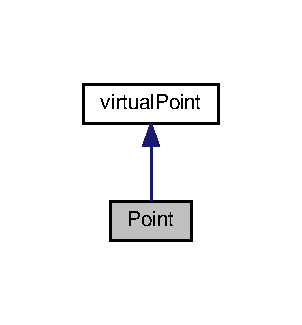
\includegraphics[width=145pt]{classPoint__inherit__graph}
\end{center}
\end{figure}


Collaboration diagram for Point\+:
\nopagebreak
\begin{figure}[H]
\begin{center}
\leavevmode
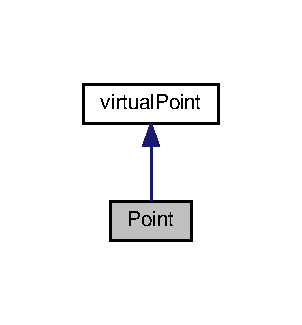
\includegraphics[width=145pt]{classPoint__coll__graph}
\end{center}
\end{figure}
\subsection*{Public Member Functions}
\begin{DoxyCompactItemize}
\item 
\hyperlink{classPoint_ad92f2337b839a94ce97dcdb439b4325a}{Point} ()
\item 
\hyperlink{classPoint_a395fa04b4ec126b66fc053f829a30cc1}{$\sim$\+Point} ()
\item 
double \hyperlink{classPoint_a7467a9db2eb234926884cf88c638da93}{get\+\_\+x} ()
\begin{DoxyCompactList}\small\item\em get\+\_\+x \end{DoxyCompactList}\item 
void \hyperlink{classPoint_a2db17626051c9c14986b40c403305c09}{set\+\_\+x} (double)
\begin{DoxyCompactList}\small\item\em set\+\_\+x \end{DoxyCompactList}\item 
double \hyperlink{classPoint_a30cce78a200b5577b03e1c9c1b1f9ad8}{get\+\_\+y} ()
\begin{DoxyCompactList}\small\item\em get\+\_\+y \end{DoxyCompactList}\item 
void \hyperlink{classPoint_a787785e71cb38bd2d3c3dece4684d89e}{set\+\_\+y} (double)
\begin{DoxyCompactList}\small\item\em set\+\_\+y \end{DoxyCompactList}\end{DoxyCompactItemize}
\subsection*{Private Attributes}
\begin{DoxyCompactItemize}
\item 
double \hyperlink{classPoint_a9a3d900d37caa93c8266045f9a15ddfd}{X}
\item 
double \hyperlink{classPoint_afd3632a85aefc15a129a8ebc4b8412b9}{Y}
\end{DoxyCompactItemize}


\subsection{Detailed Description}
class \hyperlink{classPoint}{Point} is declared with its two data members namely X and Y and four methods \+: get\+\_\+x set\+\_\+x get\+\_\+y set\+\_\+y 

\subsection{Constructor \& Destructor Documentation}
\index{Point@{Point}!Point@{Point}}
\index{Point@{Point}!Point@{Point}}
\subsubsection[{\texorpdfstring{Point()}{Point()}}]{\setlength{\rightskip}{0pt plus 5cm}Point\+::\+Point (
\begin{DoxyParamCaption}
{}
\end{DoxyParamCaption}
)}\hypertarget{classPoint_ad92f2337b839a94ce97dcdb439b4325a}{}\label{classPoint_ad92f2337b839a94ce97dcdb439b4325a}
constructor \index{Point@{Point}!````~Point@{$\sim$\+Point}}
\index{````~Point@{$\sim$\+Point}!Point@{Point}}
\subsubsection[{\texorpdfstring{$\sim$\+Point()}{~Point()}}]{\setlength{\rightskip}{0pt plus 5cm}Point\+::$\sim$\+Point (
\begin{DoxyParamCaption}
{}
\end{DoxyParamCaption}
)}\hypertarget{classPoint_a395fa04b4ec126b66fc053f829a30cc1}{}\label{classPoint_a395fa04b4ec126b66fc053f829a30cc1}
destructor 

\subsection{Member Function Documentation}
\index{Point@{Point}!get\+\_\+x@{get\+\_\+x}}
\index{get\+\_\+x@{get\+\_\+x}!Point@{Point}}
\subsubsection[{\texorpdfstring{get\+\_\+x()}{get_x()}}]{\setlength{\rightskip}{0pt plus 5cm}double Point\+::get\+\_\+x (
\begin{DoxyParamCaption}
{}
\end{DoxyParamCaption}
)\hspace{0.3cm}{\ttfamily [virtual]}}\hypertarget{classPoint_a7467a9db2eb234926884cf88c638da93}{}\label{classPoint_a7467a9db2eb234926884cf88c638da93}


get\+\_\+x 

returns the stored value of X coordinate of the the point 
\begin{DoxyParams}{Parameters}
{\em void} & \\
\hline
\end{DoxyParams}
\begin{DoxyReturn}{Returns}
double 
\end{DoxyReturn}


Implements \hyperlink{classvirtualPoint_afe6be96f2ab063515a78087d9ce22ddf}{virtual\+Point}.

\index{Point@{Point}!get\+\_\+y@{get\+\_\+y}}
\index{get\+\_\+y@{get\+\_\+y}!Point@{Point}}
\subsubsection[{\texorpdfstring{get\+\_\+y()}{get_y()}}]{\setlength{\rightskip}{0pt plus 5cm}double Point\+::get\+\_\+y (
\begin{DoxyParamCaption}
{}
\end{DoxyParamCaption}
)\hspace{0.3cm}{\ttfamily [virtual]}}\hypertarget{classPoint_a30cce78a200b5577b03e1c9c1b1f9ad8}{}\label{classPoint_a30cce78a200b5577b03e1c9c1b1f9ad8}


get\+\_\+y 

returns the stored value of Y coordinate of the the point 
\begin{DoxyParams}{Parameters}
{\em void} & \\
\hline
\end{DoxyParams}
\begin{DoxyReturn}{Returns}
double stored value of Y Coordinate from \char`\"{}\+Y\char`\"{} is returned 
\end{DoxyReturn}


Implements \hyperlink{classvirtualPoint_ab7149e207c73c324a5028c160d493ac4}{virtual\+Point}.

\index{Point@{Point}!set\+\_\+x@{set\+\_\+x}}
\index{set\+\_\+x@{set\+\_\+x}!Point@{Point}}
\subsubsection[{\texorpdfstring{set\+\_\+x(double)}{set_x(double)}}]{\setlength{\rightskip}{0pt plus 5cm}void Point\+::set\+\_\+x (
\begin{DoxyParamCaption}
\item[{double}]{x\+\_\+coordinate\+\_\+value}
\end{DoxyParamCaption}
)\hspace{0.3cm}{\ttfamily [virtual]}}\hypertarget{classPoint_a2db17626051c9c14986b40c403305c09}{}\label{classPoint_a2db17626051c9c14986b40c403305c09}


set\+\_\+x 

set the new value of X Coordinate in \char`\"{}\+X\char`\"{} datamember 
\begin{DoxyParams}{Parameters}
{\em double} & \\
\hline
\end{DoxyParams}
\begin{DoxyReturn}{Returns}
void 
\end{DoxyReturn}


Implements \hyperlink{classvirtualPoint_a2e0023f0dffbb82aee6d358a3998807d}{virtual\+Point}.

\index{Point@{Point}!set\+\_\+y@{set\+\_\+y}}
\index{set\+\_\+y@{set\+\_\+y}!Point@{Point}}
\subsubsection[{\texorpdfstring{set\+\_\+y(double)}{set_y(double)}}]{\setlength{\rightskip}{0pt plus 5cm}void Point\+::set\+\_\+y (
\begin{DoxyParamCaption}
\item[{double}]{y\+\_\+coordinate\+\_\+value}
\end{DoxyParamCaption}
)\hspace{0.3cm}{\ttfamily [virtual]}}\hypertarget{classPoint_a787785e71cb38bd2d3c3dece4684d89e}{}\label{classPoint_a787785e71cb38bd2d3c3dece4684d89e}


set\+\_\+y 

set the new value of Y Coordinate in \char`\"{}\+Y\char`\"{} datamember 
\begin{DoxyParams}{Parameters}
{\em double} & \\
\hline
\end{DoxyParams}
\begin{DoxyReturn}{Returns}
void 
\end{DoxyReturn}


Implements \hyperlink{classvirtualPoint_afbeef257f2fe3581b6f302e085968f79}{virtual\+Point}.



\subsection{Member Data Documentation}
\index{Point@{Point}!X@{X}}
\index{X@{X}!Point@{Point}}
\subsubsection[{\texorpdfstring{X}{X}}]{\setlength{\rightskip}{0pt plus 5cm}double Point\+::X\hspace{0.3cm}{\ttfamily [private]}}\hypertarget{classPoint_a9a3d900d37caa93c8266045f9a15ddfd}{}\label{classPoint_a9a3d900d37caa93c8266045f9a15ddfd}
\index{Point@{Point}!Y@{Y}}
\index{Y@{Y}!Point@{Point}}
\subsubsection[{\texorpdfstring{Y}{Y}}]{\setlength{\rightskip}{0pt plus 5cm}double Point\+::Y\hspace{0.3cm}{\ttfamily [private]}}\hypertarget{classPoint_afd3632a85aefc15a129a8ebc4b8412b9}{}\label{classPoint_afd3632a85aefc15a129a8ebc4b8412b9}


The documentation for this class was generated from the following files\+:\begin{DoxyCompactItemize}
\item 
/home/saurav/\+Documents/\+Steering Control Module/cpp-\/boilerplate/include/\hyperlink{Point_8h}{Point.\+h}\item 
/home/saurav/\+Documents/\+Steering Control Module/cpp-\/boilerplate/app/\hyperlink{Point_8cpp}{Point.\+cpp}\end{DoxyCompactItemize}

\hypertarget{classSteeringControl}{}\section{Steering\+Control Class Reference}
\label{classSteeringControl}\index{Steering\+Control@{Steering\+Control}}


class \hyperlink{classSteeringControl}{Steering\+Control} is declared with its four double type private data members (wheelbase, trackwidth, cgz, vehicle\+Velocity) and four \hyperlink{classPoint}{Point(class)}type data members (Target, Veh\+Front, Veh\+Right, Veh\+Left) class \hyperlink{classSteeringControl}{Steering\+Control} has seven methods \+: compute\+\_\+and\+\_\+update\+\_\+coordinate set\+\_\+target\+\_\+and\+\_\+veh\+\_\+velocity get\+\_\+distance has\+\_\+reached\+\_\+target, get\+\_\+front\+\_\+coordinate, get\+\_\+left\+\_\+coordinate, get\+\_\+right\+\_\+coordinate  




{\ttfamily \#include $<$Steering\+Control.\+h$>$}



Collaboration diagram for Steering\+Control\+:
\nopagebreak
\begin{figure}[H]
\begin{center}
\leavevmode
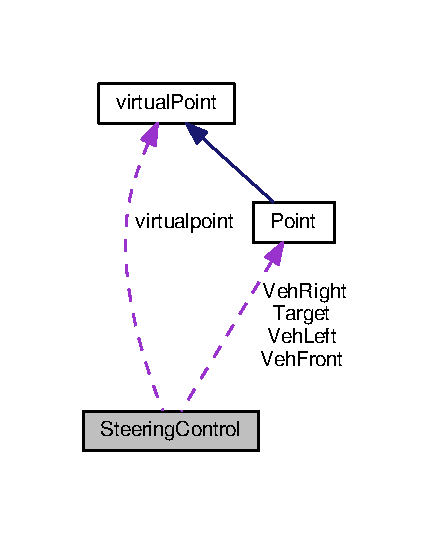
\includegraphics[width=207pt]{classSteeringControl__coll__graph}
\end{center}
\end{figure}
\subsection*{Public Member Functions}
\begin{DoxyCompactItemize}
\item 
\hyperlink{classSteeringControl_abb1f91984cfc24893b61142fb5af297f}{Steering\+Control} (\hyperlink{classvirtualPoint}{virtual\+Point} \&, double)
\begin{DoxyCompactList}\small\item\em Constructor for class \hyperlink{classSteeringControl}{Steering\+Control}. \end{DoxyCompactList}\item 
\hyperlink{classSteeringControl_a9ebb8eef465b7a1adf81271e08e34835}{$\sim$\+Steering\+Control} ()
\begin{DoxyCompactList}\small\item\em Destructor for class \hyperlink{classSteeringControl}{Steering\+Control}. \end{DoxyCompactList}\item 
\hyperlink{classSteeringControlOutput}{Steering\+Control\+Output} \hyperlink{classSteeringControl_ad4ee84da254d91ecc1811da027b4482c}{compute\+\_\+and\+\_\+update\+\_\+coordinate} ()
\begin{DoxyCompactList}\small\item\em method of the class \hyperlink{classSteeringControl}{Steering\+Control} to return the individual drive wheels velocities, steering angle and the coordinate position of the wheels after dt time period, based upon the user input of target coordinate and vehicle velocity and vehicle velocity. \end{DoxyCompactList}\item 
void \hyperlink{classSteeringControl_a6698bb99d4feccac1d9dc8c961bfaf72}{set\+\_\+vehicle\+\_\+dimension} (double, double, double)
\begin{DoxyCompactList}\small\item\em set\+\_\+vehicle\+\_\+dimension \+: takes the input from user and stores it \end{DoxyCompactList}\item 
double \hyperlink{classSteeringControl_abf86c529e73e50fa87cf25be79f3d7f4}{get\+\_\+distance} (\hyperlink{classPoint}{Point}, \hyperlink{classPoint}{Point})
\begin{DoxyCompactList}\small\item\em get\+\_\+distance \+: calculates distance \end{DoxyCompactList}\item 
bool \hyperlink{classSteeringControl_a31b1c0fe098911c1001b3c77fa65fa96}{has\+\_\+reached\+\_\+target} ()
\begin{DoxyCompactList}\small\item\em has\+\_\+reached\+\_\+target \+:checks for condition \end{DoxyCompactList}\item 
\hyperlink{classPoint}{Point} \hyperlink{classSteeringControl_a0fdca7f565d9484877850f8be65e02cc}{get\+\_\+front\+\_\+coordinate} ()
\begin{DoxyCompactList}\small\item\em get\+\_\+front\+\_\+coordinate \+: method to return front coordinate \end{DoxyCompactList}\item 
\hyperlink{classPoint}{Point} \hyperlink{classSteeringControl_a78ca3cc603867ed714dce5b792365b43}{get\+\_\+left\+\_\+coordinate} ()
\begin{DoxyCompactList}\small\item\em get\+\_\+left\+\_\+coordinate \+: method to return left coordinate \end{DoxyCompactList}\item 
\hyperlink{classPoint}{Point} \hyperlink{classSteeringControl_a5778ab49477993b2e2b586630ca08410}{get\+\_\+right\+\_\+coordinate} ()
\begin{DoxyCompactList}\small\item\em get\+\_\+right\+\_\+coordinate \+: method to return right coordinate \end{DoxyCompactList}\end{DoxyCompactItemize}
\subsection*{Private Attributes}
\begin{DoxyCompactItemize}
\item 
\hyperlink{classvirtualPoint}{virtual\+Point} \& \hyperlink{classSteeringControl_ac3008c88d68138c338a4bd3ee32e46bd}{virtualpoint}
\item 
\hyperlink{classPoint}{Point} \hyperlink{classSteeringControl_ae181dcc9db1d96ddd96ad2edcabed5b0}{Target}
\item 
double \hyperlink{classSteeringControl_aea9c0f68cdd1a1bee63712460874e54d}{vehicle\+Velocity}
\item 
double \hyperlink{classSteeringControl_a7236de7b5f030e67047cdeaea3dbabb4}{wheelbase}
\item 
double \hyperlink{classSteeringControl_a46bd4d409f6f74ecbc8dbfd44bf46b33}{trackwidth}
\item 
double \hyperlink{classSteeringControl_af9a3eafcb4395ff4bc6cc504531e8608}{cgz}
\item 
\hyperlink{classPoint}{Point} \hyperlink{classSteeringControl_a460971214c3cf817819dc261e1a48828}{Veh\+Front}
\item 
\hyperlink{classPoint}{Point} \hyperlink{classSteeringControl_a991991a5e295b9c729749c709b84f3b2}{Veh\+Right}
\item 
\hyperlink{classPoint}{Point} \hyperlink{classSteeringControl_af444dd9970b9e9872d37c601a212d78a}{Veh\+Left}
\end{DoxyCompactItemize}


\subsection{Detailed Description}
class \hyperlink{classSteeringControl}{Steering\+Control} is declared with its four double type private data members (wheelbase, trackwidth, cgz, vehicle\+Velocity) and four \hyperlink{classPoint}{Point(class)}type data members (Target, Veh\+Front, Veh\+Right, Veh\+Left) class \hyperlink{classSteeringControl}{Steering\+Control} has seven methods \+: compute\+\_\+and\+\_\+update\+\_\+coordinate set\+\_\+target\+\_\+and\+\_\+veh\+\_\+velocity get\+\_\+distance has\+\_\+reached\+\_\+target, get\+\_\+front\+\_\+coordinate, get\+\_\+left\+\_\+coordinate, get\+\_\+right\+\_\+coordinate 

\subsection{Constructor \& Destructor Documentation}
\index{Steering\+Control@{Steering\+Control}!Steering\+Control@{Steering\+Control}}
\index{Steering\+Control@{Steering\+Control}!Steering\+Control@{Steering\+Control}}
\subsubsection[{\texorpdfstring{Steering\+Control(virtual\+Point \&, double)}{SteeringControl(virtualPoint &, double)}}]{\setlength{\rightskip}{0pt plus 5cm}Steering\+Control\+::\+Steering\+Control (
\begin{DoxyParamCaption}
\item[{{\bf virtual\+Point} \&}]{vpoint, }
\item[{double}]{vehiclevelocityvalue}
\end{DoxyParamCaption}
)}\hypertarget{classSteeringControl_abb1f91984cfc24893b61142fb5af297f}{}\label{classSteeringControl_abb1f91984cfc24893b61142fb5af297f}


Constructor for class \hyperlink{classSteeringControl}{Steering\+Control}. 

constructor \index{Steering\+Control@{Steering\+Control}!````~Steering\+Control@{$\sim$\+Steering\+Control}}
\index{````~Steering\+Control@{$\sim$\+Steering\+Control}!Steering\+Control@{Steering\+Control}}
\subsubsection[{\texorpdfstring{$\sim$\+Steering\+Control()}{~SteeringControl()}}]{\setlength{\rightskip}{0pt plus 5cm}Steering\+Control\+::$\sim$\+Steering\+Control (
\begin{DoxyParamCaption}
{}
\end{DoxyParamCaption}
)}\hypertarget{classSteeringControl_a9ebb8eef465b7a1adf81271e08e34835}{}\label{classSteeringControl_a9ebb8eef465b7a1adf81271e08e34835}


Destructor for class \hyperlink{classSteeringControl}{Steering\+Control}. 

destructor 

\subsection{Member Function Documentation}
\index{Steering\+Control@{Steering\+Control}!compute\+\_\+and\+\_\+update\+\_\+coordinate@{compute\+\_\+and\+\_\+update\+\_\+coordinate}}
\index{compute\+\_\+and\+\_\+update\+\_\+coordinate@{compute\+\_\+and\+\_\+update\+\_\+coordinate}!Steering\+Control@{Steering\+Control}}
\subsubsection[{\texorpdfstring{compute\+\_\+and\+\_\+update\+\_\+coordinate()}{compute_and_update_coordinate()}}]{\setlength{\rightskip}{0pt plus 5cm}{\bf Steering\+Control\+Output} Steering\+Control\+::compute\+\_\+and\+\_\+update\+\_\+coordinate (
\begin{DoxyParamCaption}
{}
\end{DoxyParamCaption}
)}\hypertarget{classSteeringControl_ad4ee84da254d91ecc1811da027b4482c}{}\label{classSteeringControl_ad4ee84da254d91ecc1811da027b4482c}


method of the class \hyperlink{classSteeringControl}{Steering\+Control} to return the individual drive wheels velocities, steering angle and the coordinate position of the wheels after dt time period, based upon the user input of target coordinate and vehicle velocity and vehicle velocity. 

The method considers a real time latency of 0.\+01 sec.\+The first statement averages the of the left wheel coordinate and the right wheel coordinate to define a \hyperlink{classPoint}{Point(class)} Vehicle\+Axle\+Center. The \char`\"{}\+X\+Front\+Vel\+Unit\+Comp\char`\"{} computes the X component of front-\/wheel direction unit vector whereas the Y\+Front\+Vel\+Unit\+Comp calculates the Y component of front-\/wheel direction unit vector. Similarly,X\+Veh\+Orient\+Comp,Y\+Veh\+Orient\+Comp computes the X and Y component of the vehicle orientation(direction the of the front wheel from the center of the rear wheels). Veh\+Orient\+Angle and Approach\+Angle are calculated by taking tan inverse(atan2) of Y and X component of vehicle orientation and front wheel direction unit vector. A Steering angle Constraint is defined based upon the minimum value between 30 degree and the steering angle for a given velocity which can cause vehicle to tuple. The lower of two is chosen as steering angle constraint. The Steering angle is then calculated by substracting the Approach\+Angle to Veh\+Orient\+Angle. A positive value of steering angle indicates vehicle turning toward right direction (counter-\/clockwise), whereas the the negative value of the steering angle indicates vehicle turning toward left direction (clockwise direction). It is then checked whether the steering\+Angle is greater than the steering\+Angle\+Constraint. If the the magnitude of the steering angle is greater than the magnitude of steering angle constatint,the Steering\+Angle\+Constraint is set as the Steering Angle. vehicle\+Front\+Velocity is computed from the wheelbase, vehicle\+Velocity Steering\+Angle. Angular\+Velocity is computed by vehicle\+Front\+Velocity, Steering\+Angle and wheelbase. Left\+Wheel\+Speed and Right\+Wheel\+Speed is then calculated from the vehicle\+Velocity, Angular\+Velocity and the trackwidth. The coordinate of the front wheel(\+Veh\+Front) is then computed by adding the delta change after dt time to its existing value. Similarly,the coordinate of the axlecenter (Veh\+Axle\+Center) is then computed by adding the delta change after dt time to its existing value. Left\+Wheel coordinate and right wheel coordinate is then computed from the veh\+Axle\+Center, Veh\+Orient\+Angle and Angular\+Velocity. The function then returns the \hyperlink{classSteeringControlOutput}{Steering\+Control\+Output(class)} My\+Output having datamembers Left\+Wheel\+Speed, Right\+Wheel\+Speed and Steering\+Angle. 
\begin{DoxyParams}{Parameters}
{\em void} & \\
\hline
\end{DoxyParams}
\begin{DoxyReturn}{Returns}
returns the \hyperlink{classSteeringControlOutput}{Steering\+Control\+Output(class)} My\+Output having data members Left\+Wheel\+Speed, Right\+Wheel\+Speed and Steering\+Angle. 
\end{DoxyReturn}
Veh\+Orient\+Angle and Approach\+Angle is calculated

Steering\+Angle\+Constraint is calculated and implemented

vehicle\+Front\+Velocity is calculated from vehicle\+Velocity,Steering\+Angle and wheelbase

Updates the coordinates of Veh\+Front ,Veh\+Axle\+Center,Veh\+Left,Veh\+Left and Veh\+Right based on the vehiclevelocity,steering angle,orientaion angle\index{Steering\+Control@{Steering\+Control}!get\+\_\+distance@{get\+\_\+distance}}
\index{get\+\_\+distance@{get\+\_\+distance}!Steering\+Control@{Steering\+Control}}
\subsubsection[{\texorpdfstring{get\+\_\+distance(\+Point, Point)}{get_distance(Point, Point)}}]{\setlength{\rightskip}{0pt plus 5cm}double Steering\+Control\+::get\+\_\+distance (
\begin{DoxyParamCaption}
\item[{{\bf Point}}]{a, }
\item[{{\bf Point}}]{b}
\end{DoxyParamCaption}
)}\hypertarget{classSteeringControl_abf86c529e73e50fa87cf25be79f3d7f4}{}\label{classSteeringControl_abf86c529e73e50fa87cf25be79f3d7f4}


get\+\_\+distance \+: calculates distance 

calculates the distance between two Points a and b using pythagoras theorum. 
\begin{DoxyParams}{Parameters}
{\em \hyperlink{classPoint}{Point(class)}} & a having x1,y1 coordinate \\
\hline
{\em \hyperlink{classPoint}{Point(class)}} & b having x2,y2 coordinate \\
\hline
\end{DoxyParams}
\begin{DoxyReturn}{Returns}
double distance betwen the two points. 
\end{DoxyReturn}
\index{Steering\+Control@{Steering\+Control}!get\+\_\+front\+\_\+coordinate@{get\+\_\+front\+\_\+coordinate}}
\index{get\+\_\+front\+\_\+coordinate@{get\+\_\+front\+\_\+coordinate}!Steering\+Control@{Steering\+Control}}
\subsubsection[{\texorpdfstring{get\+\_\+front\+\_\+coordinate()}{get_front_coordinate()}}]{\setlength{\rightskip}{0pt plus 5cm}{\bf Point} Steering\+Control\+::get\+\_\+front\+\_\+coordinate (
\begin{DoxyParamCaption}
{}
\end{DoxyParamCaption}
)}\hypertarget{classSteeringControl_a0fdca7f565d9484877850f8be65e02cc}{}\label{classSteeringControl_a0fdca7f565d9484877850f8be65e02cc}


get\+\_\+front\+\_\+coordinate \+: method to return front coordinate 

This method of class \hyperlink{classSteeringControl}{Steering\+Control} returns the x,y coordinates of the front wheel.\+The values are passed int the vector xfront and yfront to plot the front wheel trajectory path. 
\begin{DoxyParams}{Parameters}
{\em void} & \\
\hline
\end{DoxyParams}
\begin{DoxyReturn}{Returns}
\hyperlink{classPoint}{Point(class)} Veh\+Front having two datamembers with x and y value of the front wheel 
\end{DoxyReturn}
\index{Steering\+Control@{Steering\+Control}!get\+\_\+left\+\_\+coordinate@{get\+\_\+left\+\_\+coordinate}}
\index{get\+\_\+left\+\_\+coordinate@{get\+\_\+left\+\_\+coordinate}!Steering\+Control@{Steering\+Control}}
\subsubsection[{\texorpdfstring{get\+\_\+left\+\_\+coordinate()}{get_left_coordinate()}}]{\setlength{\rightskip}{0pt plus 5cm}{\bf Point} Steering\+Control\+::get\+\_\+left\+\_\+coordinate (
\begin{DoxyParamCaption}
{}
\end{DoxyParamCaption}
)}\hypertarget{classSteeringControl_a78ca3cc603867ed714dce5b792365b43}{}\label{classSteeringControl_a78ca3cc603867ed714dce5b792365b43}


get\+\_\+left\+\_\+coordinate \+: method to return left coordinate 

This method of class \hyperlink{classSteeringControl}{Steering\+Control} returns the x,y coordinates of the left wheel.\+The values are passed int the vector xleft and yleft to plot the left wheel trajectory path. 
\begin{DoxyParams}{Parameters}
{\em void} & \\
\hline
\end{DoxyParams}
\begin{DoxyReturn}{Returns}
\hyperlink{classPoint}{Point(class)} Veh\+Left having two datamembers with x and y value of the left wheel 
\end{DoxyReturn}
\index{Steering\+Control@{Steering\+Control}!get\+\_\+right\+\_\+coordinate@{get\+\_\+right\+\_\+coordinate}}
\index{get\+\_\+right\+\_\+coordinate@{get\+\_\+right\+\_\+coordinate}!Steering\+Control@{Steering\+Control}}
\subsubsection[{\texorpdfstring{get\+\_\+right\+\_\+coordinate()}{get_right_coordinate()}}]{\setlength{\rightskip}{0pt plus 5cm}{\bf Point} Steering\+Control\+::get\+\_\+right\+\_\+coordinate (
\begin{DoxyParamCaption}
{}
\end{DoxyParamCaption}
)}\hypertarget{classSteeringControl_a5778ab49477993b2e2b586630ca08410}{}\label{classSteeringControl_a5778ab49477993b2e2b586630ca08410}


get\+\_\+right\+\_\+coordinate \+: method to return right coordinate 

This method of class \hyperlink{classSteeringControl}{Steering\+Control} returns the x,y coordinates of the right wheel.\+The values are passed int the vector xright and yright to plot the right wheel trajectory path. 
\begin{DoxyParams}{Parameters}
{\em void} & \\
\hline
\end{DoxyParams}
\begin{DoxyReturn}{Returns}
\hyperlink{classPoint}{Point(class)} Veh\+Right having two datamembers with x and y value of the right wheel 
\end{DoxyReturn}
\index{Steering\+Control@{Steering\+Control}!has\+\_\+reached\+\_\+target@{has\+\_\+reached\+\_\+target}}
\index{has\+\_\+reached\+\_\+target@{has\+\_\+reached\+\_\+target}!Steering\+Control@{Steering\+Control}}
\subsubsection[{\texorpdfstring{has\+\_\+reached\+\_\+target()}{has_reached_target()}}]{\setlength{\rightskip}{0pt plus 5cm}bool Steering\+Control\+::has\+\_\+reached\+\_\+target (
\begin{DoxyParamCaption}
{}
\end{DoxyParamCaption}
)}\hypertarget{classSteeringControl_a31b1c0fe098911c1001b3c77fa65fa96}{}\label{classSteeringControl_a31b1c0fe098911c1001b3c77fa65fa96}


has\+\_\+reached\+\_\+target \+:checks for condition 

returns true if the front wheel of the vehicle is within 1 unit radius of the defined target. 
\begin{DoxyParams}{Parameters}
{\em void} & \\
\hline
\end{DoxyParams}
\begin{DoxyReturn}{Returns}
bool 
\end{DoxyReturn}
\index{Steering\+Control@{Steering\+Control}!set\+\_\+vehicle\+\_\+dimension@{set\+\_\+vehicle\+\_\+dimension}}
\index{set\+\_\+vehicle\+\_\+dimension@{set\+\_\+vehicle\+\_\+dimension}!Steering\+Control@{Steering\+Control}}
\subsubsection[{\texorpdfstring{set\+\_\+vehicle\+\_\+dimension(double, double, double)}{set_vehicle_dimension(double, double, double)}}]{\setlength{\rightskip}{0pt plus 5cm}void Steering\+Control\+::set\+\_\+vehicle\+\_\+dimension (
\begin{DoxyParamCaption}
\item[{double}]{Wheelbase\+Value, }
\item[{double}]{Trackwidth\+Value, }
\item[{double}]{cgz\+Value}
\end{DoxyParamCaption}
)}\hypertarget{classSteeringControl_a6698bb99d4feccac1d9dc8c961bfaf72}{}\label{classSteeringControl_a6698bb99d4feccac1d9dc8c961bfaf72}


set\+\_\+vehicle\+\_\+dimension \+: takes the input from user and stores it 

Takes the three parameter and stores the value in the data members of \hyperlink{classSteeringControl}{Steering\+Control} 
\begin{DoxyParams}{Parameters}
{\em wheelbase-\/} & wheelbase of the vehile \\
\hline
{\em trackwidth} & of the vehicle \\
\hline
{\em cgz} & -\/ cgz of the vehicle \\
\hline
\end{DoxyParams}
\begin{DoxyReturn}{Returns}
void 
\end{DoxyReturn}


\subsection{Member Data Documentation}
\index{Steering\+Control@{Steering\+Control}!cgz@{cgz}}
\index{cgz@{cgz}!Steering\+Control@{Steering\+Control}}
\subsubsection[{\texorpdfstring{cgz}{cgz}}]{\setlength{\rightskip}{0pt plus 5cm}double Steering\+Control\+::cgz\hspace{0.3cm}{\ttfamily [private]}}\hypertarget{classSteeringControl_af9a3eafcb4395ff4bc6cc504531e8608}{}\label{classSteeringControl_af9a3eafcb4395ff4bc6cc504531e8608}
\index{Steering\+Control@{Steering\+Control}!Target@{Target}}
\index{Target@{Target}!Steering\+Control@{Steering\+Control}}
\subsubsection[{\texorpdfstring{Target}{Target}}]{\setlength{\rightskip}{0pt plus 5cm}{\bf Point} Steering\+Control\+::\+Target\hspace{0.3cm}{\ttfamily [private]}}\hypertarget{classSteeringControl_ae181dcc9db1d96ddd96ad2edcabed5b0}{}\label{classSteeringControl_ae181dcc9db1d96ddd96ad2edcabed5b0}
\index{Steering\+Control@{Steering\+Control}!trackwidth@{trackwidth}}
\index{trackwidth@{trackwidth}!Steering\+Control@{Steering\+Control}}
\subsubsection[{\texorpdfstring{trackwidth}{trackwidth}}]{\setlength{\rightskip}{0pt plus 5cm}double Steering\+Control\+::trackwidth\hspace{0.3cm}{\ttfamily [private]}}\hypertarget{classSteeringControl_a46bd4d409f6f74ecbc8dbfd44bf46b33}{}\label{classSteeringControl_a46bd4d409f6f74ecbc8dbfd44bf46b33}
\index{Steering\+Control@{Steering\+Control}!Veh\+Front@{Veh\+Front}}
\index{Veh\+Front@{Veh\+Front}!Steering\+Control@{Steering\+Control}}
\subsubsection[{\texorpdfstring{Veh\+Front}{VehFront}}]{\setlength{\rightskip}{0pt plus 5cm}{\bf Point} Steering\+Control\+::\+Veh\+Front\hspace{0.3cm}{\ttfamily [private]}}\hypertarget{classSteeringControl_a460971214c3cf817819dc261e1a48828}{}\label{classSteeringControl_a460971214c3cf817819dc261e1a48828}
\index{Steering\+Control@{Steering\+Control}!vehicle\+Velocity@{vehicle\+Velocity}}
\index{vehicle\+Velocity@{vehicle\+Velocity}!Steering\+Control@{Steering\+Control}}
\subsubsection[{\texorpdfstring{vehicle\+Velocity}{vehicleVelocity}}]{\setlength{\rightskip}{0pt plus 5cm}double Steering\+Control\+::vehicle\+Velocity\hspace{0.3cm}{\ttfamily [private]}}\hypertarget{classSteeringControl_aea9c0f68cdd1a1bee63712460874e54d}{}\label{classSteeringControl_aea9c0f68cdd1a1bee63712460874e54d}
\index{Steering\+Control@{Steering\+Control}!Veh\+Left@{Veh\+Left}}
\index{Veh\+Left@{Veh\+Left}!Steering\+Control@{Steering\+Control}}
\subsubsection[{\texorpdfstring{Veh\+Left}{VehLeft}}]{\setlength{\rightskip}{0pt plus 5cm}{\bf Point} Steering\+Control\+::\+Veh\+Left\hspace{0.3cm}{\ttfamily [private]}}\hypertarget{classSteeringControl_af444dd9970b9e9872d37c601a212d78a}{}\label{classSteeringControl_af444dd9970b9e9872d37c601a212d78a}
\index{Steering\+Control@{Steering\+Control}!Veh\+Right@{Veh\+Right}}
\index{Veh\+Right@{Veh\+Right}!Steering\+Control@{Steering\+Control}}
\subsubsection[{\texorpdfstring{Veh\+Right}{VehRight}}]{\setlength{\rightskip}{0pt plus 5cm}{\bf Point} Steering\+Control\+::\+Veh\+Right\hspace{0.3cm}{\ttfamily [private]}}\hypertarget{classSteeringControl_a991991a5e295b9c729749c709b84f3b2}{}\label{classSteeringControl_a991991a5e295b9c729749c709b84f3b2}
\index{Steering\+Control@{Steering\+Control}!virtualpoint@{virtualpoint}}
\index{virtualpoint@{virtualpoint}!Steering\+Control@{Steering\+Control}}
\subsubsection[{\texorpdfstring{virtualpoint}{virtualpoint}}]{\setlength{\rightskip}{0pt plus 5cm}{\bf virtual\+Point}\& Steering\+Control\+::virtualpoint\hspace{0.3cm}{\ttfamily [private]}}\hypertarget{classSteeringControl_ac3008c88d68138c338a4bd3ee32e46bd}{}\label{classSteeringControl_ac3008c88d68138c338a4bd3ee32e46bd}
\index{Steering\+Control@{Steering\+Control}!wheelbase@{wheelbase}}
\index{wheelbase@{wheelbase}!Steering\+Control@{Steering\+Control}}
\subsubsection[{\texorpdfstring{wheelbase}{wheelbase}}]{\setlength{\rightskip}{0pt plus 5cm}double Steering\+Control\+::wheelbase\hspace{0.3cm}{\ttfamily [private]}}\hypertarget{classSteeringControl_a7236de7b5f030e67047cdeaea3dbabb4}{}\label{classSteeringControl_a7236de7b5f030e67047cdeaea3dbabb4}


The documentation for this class was generated from the following files\+:\begin{DoxyCompactItemize}
\item 
/home/saurav/\+Documents/\+Steering Control Module/cpp-\/boilerplate/include/\hyperlink{SteeringControl_8h}{Steering\+Control.\+h}\item 
/home/saurav/\+Documents/\+Steering Control Module/cpp-\/boilerplate/app/\hyperlink{SteeringControl_8cpp}{Steering\+Control.\+cpp}\end{DoxyCompactItemize}

\hypertarget{classSteeringControlOutput}{}\section{Steering\+Control\+Output Class Reference}
\label{classSteeringControlOutput}\index{Steering\+Control\+Output@{Steering\+Control\+Output}}


class \hyperlink{classSteeringControlOutput}{Steering\+Control\+Output} is declared with its three data members namely Left\+Wheel\+Speed, Right\+Wheel\+Speed and Steering\+Angle and have six methods \+: get\+\_\+left\+\_\+wheel\+\_\+speed set\+\_\+left\+\_\+wheel\+\_\+speed get\+\_\+right\+\_\+wheel\+\_\+speed set\+\_\+right\+\_\+wheel\+\_\+speed get\+\_\+steering\+\_\+angle set\+\_\+steering\+\_\+angle  




{\ttfamily \#include $<$Steering\+Control\+Output.\+h$>$}

\subsection*{Public Member Functions}
\begin{DoxyCompactItemize}
\item 
\hyperlink{classSteeringControlOutput_a7e9875f06445d4e8b9773b5507755fd6}{Steering\+Control\+Output} ()
\item 
\hyperlink{classSteeringControlOutput_a2c068ac47368fae97f2a66fd11655372}{$\sim$\+Steering\+Control\+Output} ()
\item 
double \hyperlink{classSteeringControlOutput_af49e9f149fbdf2a5266e432acf9f81be}{get\+\_\+left\+\_\+wheel\+\_\+speed} ()
\begin{DoxyCompactList}\small\item\em get\+\_\+left\+\_\+wheel\+\_\+speed \end{DoxyCompactList}\item 
void \hyperlink{classSteeringControlOutput_a79f350659080a988e4df4174f849b98e}{set\+\_\+left\+\_\+wheel\+\_\+speed} (double)
\begin{DoxyCompactList}\small\item\em set\+\_\+left\+\_\+wheel\+\_\+speed \+: stores the new value for left wheel speed \end{DoxyCompactList}\item 
double \hyperlink{classSteeringControlOutput_a44153ca072242f333327dd36dd358b88}{get\+\_\+right\+\_\+wheel\+\_\+speed} ()
\begin{DoxyCompactList}\small\item\em get\+\_\+left\+\_\+wheel\+\_\+speed \+: returns the stored value of right wheel speed \end{DoxyCompactList}\item 
void \hyperlink{classSteeringControlOutput_af714d4bfb1234cf4b44e1231ed181da2}{set\+\_\+right\+\_\+wheel\+\_\+speed} (double)
\begin{DoxyCompactList}\small\item\em set\+\_\+right\+\_\+wheel\+\_\+speed \+: stores the new value for right wheel speed \end{DoxyCompactList}\item 
double \hyperlink{classSteeringControlOutput_a8d39c27f9056b1c887c2efa1698a7d8f}{get\+\_\+steering\+\_\+angle} ()
\begin{DoxyCompactList}\small\item\em get\+\_\+steering\+\_\+angle \end{DoxyCompactList}\item 
void \hyperlink{classSteeringControlOutput_a6dcbb32a6b426b785045fb3ddb17a840}{set\+\_\+steering\+\_\+angle} (double)
\begin{DoxyCompactList}\small\item\em set\+\_\+steering\+\_\+angle \+: stores the new value for steering angle \end{DoxyCompactList}\end{DoxyCompactItemize}
\subsection*{Private Attributes}
\begin{DoxyCompactItemize}
\item 
double \hyperlink{classSteeringControlOutput_a298c15a49cae72dc24dc692d7c02a202}{Left\+Wheel\+Speed}
\item 
double \hyperlink{classSteeringControlOutput_accc25fe9c42570d6a42517be19cd4229}{Right\+Wheel\+Speed}
\item 
double \hyperlink{classSteeringControlOutput_aa13642c9701cdb34c8013dab7f475baf}{Steering\+Angle}
\end{DoxyCompactItemize}


\subsection{Detailed Description}
class \hyperlink{classSteeringControlOutput}{Steering\+Control\+Output} is declared with its three data members namely Left\+Wheel\+Speed, Right\+Wheel\+Speed and Steering\+Angle and have six methods \+: get\+\_\+left\+\_\+wheel\+\_\+speed set\+\_\+left\+\_\+wheel\+\_\+speed get\+\_\+right\+\_\+wheel\+\_\+speed set\+\_\+right\+\_\+wheel\+\_\+speed get\+\_\+steering\+\_\+angle set\+\_\+steering\+\_\+angle 

\subsection{Constructor \& Destructor Documentation}
\index{Steering\+Control\+Output@{Steering\+Control\+Output}!Steering\+Control\+Output@{Steering\+Control\+Output}}
\index{Steering\+Control\+Output@{Steering\+Control\+Output}!Steering\+Control\+Output@{Steering\+Control\+Output}}
\subsubsection[{\texorpdfstring{Steering\+Control\+Output()}{SteeringControlOutput()}}]{\setlength{\rightskip}{0pt plus 5cm}Steering\+Control\+Output\+::\+Steering\+Control\+Output (
\begin{DoxyParamCaption}
{}
\end{DoxyParamCaption}
)}\hypertarget{classSteeringControlOutput_a7e9875f06445d4e8b9773b5507755fd6}{}\label{classSteeringControlOutput_a7e9875f06445d4e8b9773b5507755fd6}
constructor \index{Steering\+Control\+Output@{Steering\+Control\+Output}!````~Steering\+Control\+Output@{$\sim$\+Steering\+Control\+Output}}
\index{````~Steering\+Control\+Output@{$\sim$\+Steering\+Control\+Output}!Steering\+Control\+Output@{Steering\+Control\+Output}}
\subsubsection[{\texorpdfstring{$\sim$\+Steering\+Control\+Output()}{~SteeringControlOutput()}}]{\setlength{\rightskip}{0pt plus 5cm}Steering\+Control\+Output\+::$\sim$\+Steering\+Control\+Output (
\begin{DoxyParamCaption}
{}
\end{DoxyParamCaption}
)}\hypertarget{classSteeringControlOutput_a2c068ac47368fae97f2a66fd11655372}{}\label{classSteeringControlOutput_a2c068ac47368fae97f2a66fd11655372}
destructor 

\subsection{Member Function Documentation}
\index{Steering\+Control\+Output@{Steering\+Control\+Output}!get\+\_\+left\+\_\+wheel\+\_\+speed@{get\+\_\+left\+\_\+wheel\+\_\+speed}}
\index{get\+\_\+left\+\_\+wheel\+\_\+speed@{get\+\_\+left\+\_\+wheel\+\_\+speed}!Steering\+Control\+Output@{Steering\+Control\+Output}}
\subsubsection[{\texorpdfstring{get\+\_\+left\+\_\+wheel\+\_\+speed()}{get_left_wheel_speed()}}]{\setlength{\rightskip}{0pt plus 5cm}double Steering\+Control\+Output\+::get\+\_\+left\+\_\+wheel\+\_\+speed (
\begin{DoxyParamCaption}
{}
\end{DoxyParamCaption}
)}\hypertarget{classSteeringControlOutput_af49e9f149fbdf2a5266e432acf9f81be}{}\label{classSteeringControlOutput_af49e9f149fbdf2a5266e432acf9f81be}


get\+\_\+left\+\_\+wheel\+\_\+speed 

returns the stored value of left wheel speed 
\begin{DoxyParams}{Parameters}
{\em void} & \\
\hline
\end{DoxyParams}
\begin{DoxyReturn}{Returns}
double stored value of left wheel speed from \char`\"{}\+Left\+Wheel\+Speed\char`\"{} is returned 
\end{DoxyReturn}
\index{Steering\+Control\+Output@{Steering\+Control\+Output}!get\+\_\+right\+\_\+wheel\+\_\+speed@{get\+\_\+right\+\_\+wheel\+\_\+speed}}
\index{get\+\_\+right\+\_\+wheel\+\_\+speed@{get\+\_\+right\+\_\+wheel\+\_\+speed}!Steering\+Control\+Output@{Steering\+Control\+Output}}
\subsubsection[{\texorpdfstring{get\+\_\+right\+\_\+wheel\+\_\+speed()}{get_right_wheel_speed()}}]{\setlength{\rightskip}{0pt plus 5cm}double Steering\+Control\+Output\+::get\+\_\+right\+\_\+wheel\+\_\+speed (
\begin{DoxyParamCaption}
{}
\end{DoxyParamCaption}
)}\hypertarget{classSteeringControlOutput_a44153ca072242f333327dd36dd358b88}{}\label{classSteeringControlOutput_a44153ca072242f333327dd36dd358b88}


get\+\_\+left\+\_\+wheel\+\_\+speed \+: returns the stored value of right wheel speed 

returns the stored value of right wheel speed 
\begin{DoxyParams}{Parameters}
{\em void} & \\
\hline
\end{DoxyParams}
\begin{DoxyReturn}{Returns}
double stored value of right wheel speed from \char`\"{}\+Rightt\+Wheel\+Speed\char`\"{} is returned. 
\end{DoxyReturn}
\index{Steering\+Control\+Output@{Steering\+Control\+Output}!get\+\_\+steering\+\_\+angle@{get\+\_\+steering\+\_\+angle}}
\index{get\+\_\+steering\+\_\+angle@{get\+\_\+steering\+\_\+angle}!Steering\+Control\+Output@{Steering\+Control\+Output}}
\subsubsection[{\texorpdfstring{get\+\_\+steering\+\_\+angle()}{get_steering_angle()}}]{\setlength{\rightskip}{0pt plus 5cm}double Steering\+Control\+Output\+::get\+\_\+steering\+\_\+angle (
\begin{DoxyParamCaption}
{}
\end{DoxyParamCaption}
)}\hypertarget{classSteeringControlOutput_a8d39c27f9056b1c887c2efa1698a7d8f}{}\label{classSteeringControlOutput_a8d39c27f9056b1c887c2efa1698a7d8f}


get\+\_\+steering\+\_\+angle 

returns the stored value of steering angle in radians 
\begin{DoxyParams}{Parameters}
{\em void} & \\
\hline
\end{DoxyParams}
\begin{DoxyReturn}{Returns}
double stored value of steering angle from \char`\"{}\+Steering\+Angle\char`\"{} is returned 
\end{DoxyReturn}
\index{Steering\+Control\+Output@{Steering\+Control\+Output}!set\+\_\+left\+\_\+wheel\+\_\+speed@{set\+\_\+left\+\_\+wheel\+\_\+speed}}
\index{set\+\_\+left\+\_\+wheel\+\_\+speed@{set\+\_\+left\+\_\+wheel\+\_\+speed}!Steering\+Control\+Output@{Steering\+Control\+Output}}
\subsubsection[{\texorpdfstring{set\+\_\+left\+\_\+wheel\+\_\+speed(double)}{set_left_wheel_speed(double)}}]{\setlength{\rightskip}{0pt plus 5cm}void Steering\+Control\+Output\+::set\+\_\+left\+\_\+wheel\+\_\+speed (
\begin{DoxyParamCaption}
\item[{double}]{left\+\_\+speed\+\_\+speed\+\_\+value}
\end{DoxyParamCaption}
)}\hypertarget{classSteeringControlOutput_a79f350659080a988e4df4174f849b98e}{}\label{classSteeringControlOutput_a79f350659080a988e4df4174f849b98e}


set\+\_\+left\+\_\+wheel\+\_\+speed \+: stores the new value for left wheel speed 

stores the new value of left wheel speed in \char`\"{}\+Left\+Wheel\+Speed\char`\"{}. 
\begin{DoxyParams}{Parameters}
{\em double} & \\
\hline
\end{DoxyParams}
\begin{DoxyReturn}{Returns}
void 
\end{DoxyReturn}
\index{Steering\+Control\+Output@{Steering\+Control\+Output}!set\+\_\+right\+\_\+wheel\+\_\+speed@{set\+\_\+right\+\_\+wheel\+\_\+speed}}
\index{set\+\_\+right\+\_\+wheel\+\_\+speed@{set\+\_\+right\+\_\+wheel\+\_\+speed}!Steering\+Control\+Output@{Steering\+Control\+Output}}
\subsubsection[{\texorpdfstring{set\+\_\+right\+\_\+wheel\+\_\+speed(double)}{set_right_wheel_speed(double)}}]{\setlength{\rightskip}{0pt plus 5cm}void Steering\+Control\+Output\+::set\+\_\+right\+\_\+wheel\+\_\+speed (
\begin{DoxyParamCaption}
\item[{double}]{right\+\_\+speed\+\_\+speed\+\_\+value}
\end{DoxyParamCaption}
)}\hypertarget{classSteeringControlOutput_af714d4bfb1234cf4b44e1231ed181da2}{}\label{classSteeringControlOutput_af714d4bfb1234cf4b44e1231ed181da2}


set\+\_\+right\+\_\+wheel\+\_\+speed \+: stores the new value for right wheel speed 

stores the new value of right wheel speed in \char`\"{}right\+Wheel\+Speed\char`\"{}. 
\begin{DoxyParams}{Parameters}
{\em double} & \\
\hline
\end{DoxyParams}
\begin{DoxyReturn}{Returns}
void 
\end{DoxyReturn}
\index{Steering\+Control\+Output@{Steering\+Control\+Output}!set\+\_\+steering\+\_\+angle@{set\+\_\+steering\+\_\+angle}}
\index{set\+\_\+steering\+\_\+angle@{set\+\_\+steering\+\_\+angle}!Steering\+Control\+Output@{Steering\+Control\+Output}}
\subsubsection[{\texorpdfstring{set\+\_\+steering\+\_\+angle(double)}{set_steering_angle(double)}}]{\setlength{\rightskip}{0pt plus 5cm}void Steering\+Control\+Output\+::set\+\_\+steering\+\_\+angle (
\begin{DoxyParamCaption}
\item[{double}]{steering\+\_\+angle\+\_\+value}
\end{DoxyParamCaption}
)}\hypertarget{classSteeringControlOutput_a6dcbb32a6b426b785045fb3ddb17a840}{}\label{classSteeringControlOutput_a6dcbb32a6b426b785045fb3ddb17a840}


set\+\_\+steering\+\_\+angle \+: stores the new value for steering angle 

stores the new value of steering angle in \char`\"{}\+Steering\+Angle\char`\"{}. 
\begin{DoxyParams}{Parameters}
{\em double} & \\
\hline
\end{DoxyParams}
\begin{DoxyReturn}{Returns}
void 
\end{DoxyReturn}


\subsection{Member Data Documentation}
\index{Steering\+Control\+Output@{Steering\+Control\+Output}!Left\+Wheel\+Speed@{Left\+Wheel\+Speed}}
\index{Left\+Wheel\+Speed@{Left\+Wheel\+Speed}!Steering\+Control\+Output@{Steering\+Control\+Output}}
\subsubsection[{\texorpdfstring{Left\+Wheel\+Speed}{LeftWheelSpeed}}]{\setlength{\rightskip}{0pt plus 5cm}double Steering\+Control\+Output\+::\+Left\+Wheel\+Speed\hspace{0.3cm}{\ttfamily [private]}}\hypertarget{classSteeringControlOutput_a298c15a49cae72dc24dc692d7c02a202}{}\label{classSteeringControlOutput_a298c15a49cae72dc24dc692d7c02a202}
\index{Steering\+Control\+Output@{Steering\+Control\+Output}!Right\+Wheel\+Speed@{Right\+Wheel\+Speed}}
\index{Right\+Wheel\+Speed@{Right\+Wheel\+Speed}!Steering\+Control\+Output@{Steering\+Control\+Output}}
\subsubsection[{\texorpdfstring{Right\+Wheel\+Speed}{RightWheelSpeed}}]{\setlength{\rightskip}{0pt plus 5cm}double Steering\+Control\+Output\+::\+Right\+Wheel\+Speed\hspace{0.3cm}{\ttfamily [private]}}\hypertarget{classSteeringControlOutput_accc25fe9c42570d6a42517be19cd4229}{}\label{classSteeringControlOutput_accc25fe9c42570d6a42517be19cd4229}
\index{Steering\+Control\+Output@{Steering\+Control\+Output}!Steering\+Angle@{Steering\+Angle}}
\index{Steering\+Angle@{Steering\+Angle}!Steering\+Control\+Output@{Steering\+Control\+Output}}
\subsubsection[{\texorpdfstring{Steering\+Angle}{SteeringAngle}}]{\setlength{\rightskip}{0pt plus 5cm}double Steering\+Control\+Output\+::\+Steering\+Angle\hspace{0.3cm}{\ttfamily [private]}}\hypertarget{classSteeringControlOutput_aa13642c9701cdb34c8013dab7f475baf}{}\label{classSteeringControlOutput_aa13642c9701cdb34c8013dab7f475baf}


The documentation for this class was generated from the following files\+:\begin{DoxyCompactItemize}
\item 
/home/saurav/\+Documents/\+Steering Control Module/cpp-\/boilerplate/include/\hyperlink{SteeringControlOutput_8h}{Steering\+Control\+Output.\+h}\item 
/home/saurav/\+Documents/\+Steering Control Module/cpp-\/boilerplate/app/\hyperlink{SteeringControlOutput_8cpp}{Steering\+Control\+Output.\+cpp}\end{DoxyCompactItemize}

\hypertarget{classvirtualPoint}{}\section{virtual\+Point Class Reference}
\label{classvirtualPoint}\index{virtual\+Point@{virtual\+Point}}


{\ttfamily \#include $<$virtual\+Point.\+h$>$}



Inheritance diagram for virtual\+Point\+:
\nopagebreak
\begin{figure}[H]
\begin{center}
\leavevmode
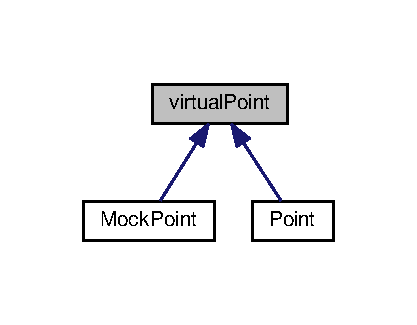
\includegraphics[width=200pt]{classvirtualPoint__inherit__graph}
\end{center}
\end{figure}
\subsection*{Public Member Functions}
\begin{DoxyCompactItemize}
\item 
virtual \hyperlink{classvirtualPoint_a4f78d9a654861eb4bec3c9acd4b00c24}{$\sim$virtual\+Point} ()
\item 
virtual double \hyperlink{classvirtualPoint_afe6be96f2ab063515a78087d9ce22ddf}{get\+\_\+x} ()=0
\begin{DoxyCompactList}\small\item\em get\+\_\+x \end{DoxyCompactList}\item 
virtual void \hyperlink{classvirtualPoint_a2e0023f0dffbb82aee6d358a3998807d}{set\+\_\+x} (double x\+\_\+coordinate\+\_\+value)=0
\begin{DoxyCompactList}\small\item\em set\+\_\+x \end{DoxyCompactList}\item 
virtual double \hyperlink{classvirtualPoint_ab7149e207c73c324a5028c160d493ac4}{get\+\_\+y} ()=0
\begin{DoxyCompactList}\small\item\em get\+\_\+y \end{DoxyCompactList}\item 
virtual void \hyperlink{classvirtualPoint_afbeef257f2fe3581b6f302e085968f79}{set\+\_\+y} (double y\+\_\+coordinate\+\_\+value)=0
\begin{DoxyCompactList}\small\item\em set\+\_\+y \end{DoxyCompactList}\end{DoxyCompactItemize}


\subsection{Constructor \& Destructor Documentation}
\index{virtual\+Point@{virtual\+Point}!````~virtual\+Point@{$\sim$virtual\+Point}}
\index{````~virtual\+Point@{$\sim$virtual\+Point}!virtual\+Point@{virtual\+Point}}
\subsubsection[{\texorpdfstring{$\sim$virtual\+Point()}{~virtualPoint()}}]{\setlength{\rightskip}{0pt plus 5cm}virtual virtual\+Point\+::$\sim$virtual\+Point (
\begin{DoxyParamCaption}
{}
\end{DoxyParamCaption}
)\hspace{0.3cm}{\ttfamily [inline]}, {\ttfamily [virtual]}}\hypertarget{classvirtualPoint_a4f78d9a654861eb4bec3c9acd4b00c24}{}\label{classvirtualPoint_a4f78d9a654861eb4bec3c9acd4b00c24}
constructor destructor 

\subsection{Member Function Documentation}
\index{virtual\+Point@{virtual\+Point}!get\+\_\+x@{get\+\_\+x}}
\index{get\+\_\+x@{get\+\_\+x}!virtual\+Point@{virtual\+Point}}
\subsubsection[{\texorpdfstring{get\+\_\+x()=0}{get_x()=0}}]{\setlength{\rightskip}{0pt plus 5cm}virtual double virtual\+Point\+::get\+\_\+x (
\begin{DoxyParamCaption}
{}
\end{DoxyParamCaption}
)\hspace{0.3cm}{\ttfamily [pure virtual]}}\hypertarget{classvirtualPoint_afe6be96f2ab063515a78087d9ce22ddf}{}\label{classvirtualPoint_afe6be96f2ab063515a78087d9ce22ddf}


get\+\_\+x 

returns the stored value of X coordinate of the the point 
\begin{DoxyParams}{Parameters}
{\em void} & \\
\hline
\end{DoxyParams}
\begin{DoxyReturn}{Returns}
double 
\end{DoxyReturn}


Implemented in \hyperlink{classPoint_a7467a9db2eb234926884cf88c638da93}{Point}.

\index{virtual\+Point@{virtual\+Point}!get\+\_\+y@{get\+\_\+y}}
\index{get\+\_\+y@{get\+\_\+y}!virtual\+Point@{virtual\+Point}}
\subsubsection[{\texorpdfstring{get\+\_\+y()=0}{get_y()=0}}]{\setlength{\rightskip}{0pt plus 5cm}virtual double virtual\+Point\+::get\+\_\+y (
\begin{DoxyParamCaption}
{}
\end{DoxyParamCaption}
)\hspace{0.3cm}{\ttfamily [pure virtual]}}\hypertarget{classvirtualPoint_ab7149e207c73c324a5028c160d493ac4}{}\label{classvirtualPoint_ab7149e207c73c324a5028c160d493ac4}


get\+\_\+y 

returns the stored value of Y coordinate of the the point 
\begin{DoxyParams}{Parameters}
{\em void} & \\
\hline
\end{DoxyParams}
\begin{DoxyReturn}{Returns}
double stored value of Y Coordinate from \char`\"{}\+Y\char`\"{} is returned 
\end{DoxyReturn}


Implemented in \hyperlink{classPoint_a30cce78a200b5577b03e1c9c1b1f9ad8}{Point}.

\index{virtual\+Point@{virtual\+Point}!set\+\_\+x@{set\+\_\+x}}
\index{set\+\_\+x@{set\+\_\+x}!virtual\+Point@{virtual\+Point}}
\subsubsection[{\texorpdfstring{set\+\_\+x(double x\+\_\+coordinate\+\_\+value)=0}{set_x(double x_coordinate_value)=0}}]{\setlength{\rightskip}{0pt plus 5cm}virtual void virtual\+Point\+::set\+\_\+x (
\begin{DoxyParamCaption}
\item[{double}]{x\+\_\+coordinate\+\_\+value}
\end{DoxyParamCaption}
)\hspace{0.3cm}{\ttfamily [pure virtual]}}\hypertarget{classvirtualPoint_a2e0023f0dffbb82aee6d358a3998807d}{}\label{classvirtualPoint_a2e0023f0dffbb82aee6d358a3998807d}


set\+\_\+x 

set the new value of X Coordinate in \char`\"{}\+X\char`\"{} datamember 
\begin{DoxyParams}{Parameters}
{\em double} & \\
\hline
\end{DoxyParams}
\begin{DoxyReturn}{Returns}
void 
\end{DoxyReturn}


Implemented in \hyperlink{classPoint_a2db17626051c9c14986b40c403305c09}{Point}.

\index{virtual\+Point@{virtual\+Point}!set\+\_\+y@{set\+\_\+y}}
\index{set\+\_\+y@{set\+\_\+y}!virtual\+Point@{virtual\+Point}}
\subsubsection[{\texorpdfstring{set\+\_\+y(double y\+\_\+coordinate\+\_\+value)=0}{set_y(double y_coordinate_value)=0}}]{\setlength{\rightskip}{0pt plus 5cm}virtual void virtual\+Point\+::set\+\_\+y (
\begin{DoxyParamCaption}
\item[{double}]{y\+\_\+coordinate\+\_\+value}
\end{DoxyParamCaption}
)\hspace{0.3cm}{\ttfamily [pure virtual]}}\hypertarget{classvirtualPoint_afbeef257f2fe3581b6f302e085968f79}{}\label{classvirtualPoint_afbeef257f2fe3581b6f302e085968f79}


set\+\_\+y 

set the new value of Y Coordinate in \char`\"{}\+Y\char`\"{} datamember 
\begin{DoxyParams}{Parameters}
{\em double} & \\
\hline
\end{DoxyParams}
\begin{DoxyReturn}{Returns}
void 
\end{DoxyReturn}


Implemented in \hyperlink{classPoint_a787785e71cb38bd2d3c3dece4684d89e}{Point}.



The documentation for this class was generated from the following file\+:\begin{DoxyCompactItemize}
\item 
/home/saurav/\+Documents/\+Steering Control Module/cpp-\/boilerplate/include/\hyperlink{virtualPoint_8h}{virtual\+Point.\+h}\end{DoxyCompactItemize}

\chapter{File Documentation}
\hypertarget{app_2main_8cpp}{}\section{/home/saurav/\+Documents/\+Steering Control Module/cpp-\/boilerplate/app/main.cpp File Reference}
\label{app_2main_8cpp}\index{/home/saurav/\+Documents/\+Steering Control Module/cpp-\/boilerplate/app/main.\+cpp@{/home/saurav/\+Documents/\+Steering Control Module/cpp-\/boilerplate/app/main.\+cpp}}


Takes target coordinate and vehicle velocity as input and provides individual wheel speed and steering angle as output until the vehicle has reached the defined target coordinate.  


{\ttfamily \#include $<$iostream$>$}\\*
{\ttfamily \#include $<$vector$>$}\\*
{\ttfamily \#include \char`\"{}../include/\+Steering\+Control.\+h\char`\"{}}\\*
Include dependency graph for main.\+cpp\+:
\nopagebreak
\begin{figure}[H]
\begin{center}
\leavevmode
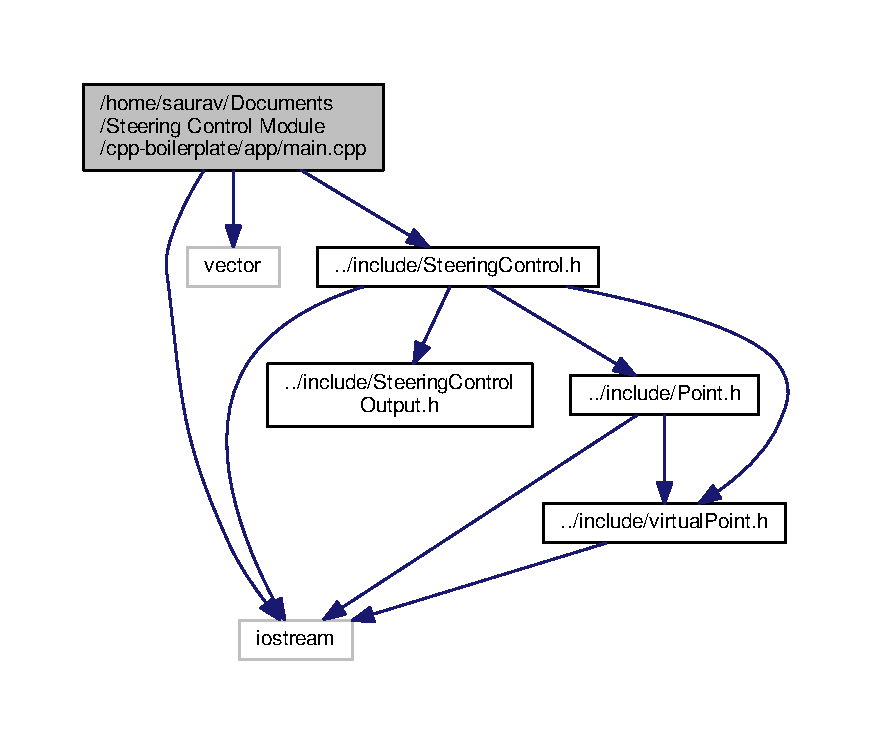
\includegraphics[width=350pt]{app_2main_8cpp__incl}
\end{center}
\end{figure}
\subsection*{Macros}
\begin{DoxyCompactItemize}
\item 
\#define \hyperlink{app_2main_8cpp_a598a3330b3c21701223ee0ca14316eca}{PI}~3.\+14159265
\end{DoxyCompactItemize}
\subsection*{Functions}
\begin{DoxyCompactItemize}
\item 
int \hyperlink{app_2main_8cpp_ae66f6b31b5ad750f1fe042a706a4e3d4}{main} ()
\end{DoxyCompactItemize}


\subsection{Detailed Description}
Takes target coordinate and vehicle velocity as input and provides individual wheel speed and steering angle as output until the vehicle has reached the defined target coordinate. 

\begin{DoxyAuthor}{Author}
Saurav Kumar 
\end{DoxyAuthor}
\begin{DoxyCopyright}{Copyright}
2018
\end{DoxyCopyright}
B\+SD 3-\/\+Clause License

Copyright (c) 2018, Saurav Kumar All rights reserved.

Redistribution and use in source and binary forms, with or without modification, are permitted provided that the following conditions are met\+:

Redistributions of source code must retain the above copyright notice, this list of conditions and the following disclaimer.

Redistributions in binary form must reproduce the above copyright notice, this list of conditions and the following disclaimer in the documentation and/or other materials provided with the distribution.

Neither the name of the copyright holder nor the names of its contributors may be used to endorse or promote products derived from this software without specific prior written permission.

T\+H\+IS S\+O\+F\+T\+W\+A\+RE IS P\+R\+O\+V\+I\+D\+ED BY T\+HE C\+O\+P\+Y\+R\+I\+G\+HT H\+O\+L\+D\+E\+RS A\+ND C\+O\+N\+T\+R\+I\+B\+U\+T\+O\+RS \char`\"{}\+A\+S I\+S\char`\"{} A\+ND A\+NY E\+X\+P\+R\+E\+SS OR I\+M\+P\+L\+I\+ED W\+A\+R\+R\+A\+N\+T\+I\+ES, I\+N\+C\+L\+U\+D\+I\+NG, B\+UT N\+OT L\+I\+M\+I\+T\+ED TO, T\+HE I\+M\+P\+L\+I\+ED W\+A\+R\+R\+A\+N\+T\+I\+ES OF M\+E\+R\+C\+H\+A\+N\+T\+A\+B\+I\+L\+I\+TY A\+ND F\+I\+T\+N\+E\+SS F\+OR A P\+A\+R\+T\+I\+C\+U\+L\+AR P\+U\+R\+P\+O\+SE A\+RE D\+I\+S\+C\+L\+A\+I\+M\+ED. IN NO E\+V\+E\+NT S\+H\+A\+LL T\+HE C\+O\+P\+Y\+R\+I\+G\+HT H\+O\+L\+D\+ER OR C\+O\+N\+T\+R\+I\+B\+U\+T\+O\+RS BE L\+I\+A\+B\+LE F\+OR A\+NY D\+I\+R\+E\+CT, I\+N\+D\+I\+R\+E\+CT, I\+N\+C\+I\+D\+E\+N\+T\+AL, S\+P\+E\+C\+I\+AL, E\+X\+E\+M\+P\+L\+A\+RY, OR C\+O\+N\+S\+E\+Q\+U\+E\+N\+T\+I\+AL D\+A\+M\+A\+G\+ES (I\+N\+C\+L\+U\+D\+I\+NG, B\+UT N\+OT L\+I\+M\+I\+T\+ED TO, P\+R\+O\+C\+U\+R\+E\+M\+E\+NT OF S\+U\+B\+S\+T\+I\+T\+U\+TE G\+O\+O\+DS OR S\+E\+R\+V\+I\+C\+ES; L\+O\+SS OF U\+SE, D\+A\+TA, OR P\+R\+O\+F\+I\+TS; OR B\+U\+S\+I\+N\+E\+SS I\+N\+T\+E\+R\+R\+U\+P\+T\+I\+ON) H\+O\+W\+E\+V\+ER C\+A\+U\+S\+ED A\+ND ON A\+NY T\+H\+E\+O\+RY OF L\+I\+A\+B\+I\+L\+I\+TY, W\+H\+E\+T\+H\+ER IN C\+O\+N\+T\+R\+A\+CT, S\+T\+R\+I\+CT L\+I\+A\+B\+I\+L\+I\+TY, OR T\+O\+RT (I\+N\+C\+L\+U\+D\+I\+NG N\+E\+G\+L\+I\+G\+E\+N\+CE OR O\+T\+H\+E\+R\+W\+I\+SE) A\+R\+I\+S\+I\+NG IN A\+NY W\+AY O\+UT OF T\+HE U\+SE OF T\+H\+IS S\+O\+F\+T\+W\+A\+RE, E\+V\+EN IF A\+D\+V\+I\+S\+ED OF T\+HE P\+O\+S\+S\+I\+B\+I\+L\+I\+TY OF S\+U\+CH D\+A\+M\+A\+GE. 

\subsection{Macro Definition Documentation}
\index{app/main.\+cpp@{app/main.\+cpp}!PI@{PI}}
\index{PI@{PI}!app/main.\+cpp@{app/main.\+cpp}}
\subsubsection[{\texorpdfstring{PI}{PI}}]{\setlength{\rightskip}{0pt plus 5cm}\#define PI~3.\+14159265}\hypertarget{app_2main_8cpp_a598a3330b3c21701223ee0ca14316eca}{}\label{app_2main_8cpp_a598a3330b3c21701223ee0ca14316eca}


\subsection{Function Documentation}
\index{app/main.\+cpp@{app/main.\+cpp}!main@{main}}
\index{main@{main}!app/main.\+cpp@{app/main.\+cpp}}
\subsubsection[{\texorpdfstring{main()}{main()}}]{\setlength{\rightskip}{0pt plus 5cm}int main (
\begin{DoxyParamCaption}
{}
\end{DoxyParamCaption}
)}\hypertarget{app_2main_8cpp_ae66f6b31b5ad750f1fe042a706a4e3d4}{}\label{app_2main_8cpp_ae66f6b31b5ad750f1fe042a706a4e3d4}
Takes the details of the vehicle parameters such as wheelbase, trackwitdh and the height of center of gravity along with the target coordinate and the vehicle velocity

An object is called of class \hyperlink{classSteeringControl}{Steering\+Control} and its parameters are fed

Target and the vehicle velocity is set for the object Vehicle which is taken as input.

Loop is run to until the vehicle reach the target coordinate
\hypertarget{demo_2main_8cpp}{}\section{/home/saurav/\+Documents/\+Steering Control Module/cpp-\/boilerplate/demo/main.cpp File Reference}
\label{demo_2main_8cpp}\index{/home/saurav/\+Documents/\+Steering Control Module/cpp-\/boilerplate/demo/main.\+cpp@{/home/saurav/\+Documents/\+Steering Control Module/cpp-\/boilerplate/demo/main.\+cpp}}


Takes target coordinate and vehicle velocity as input and provides individual wheel speed and steering angle as output untill the vehicle has reached the defined target coordinate. It also prints the and speed of individual drive wheels,steering angle in degree and the coorinates of wheel ends .  


{\ttfamily \#include $<$iostream$>$}\\*
{\ttfamily \#include $<$vector$>$}\\*
{\ttfamily \#include \char`\"{}../include/\+Steering\+Control.\+h\char`\"{}}\\*
Include dependency graph for main.\+cpp\+:
\nopagebreak
\begin{figure}[H]
\begin{center}
\leavevmode
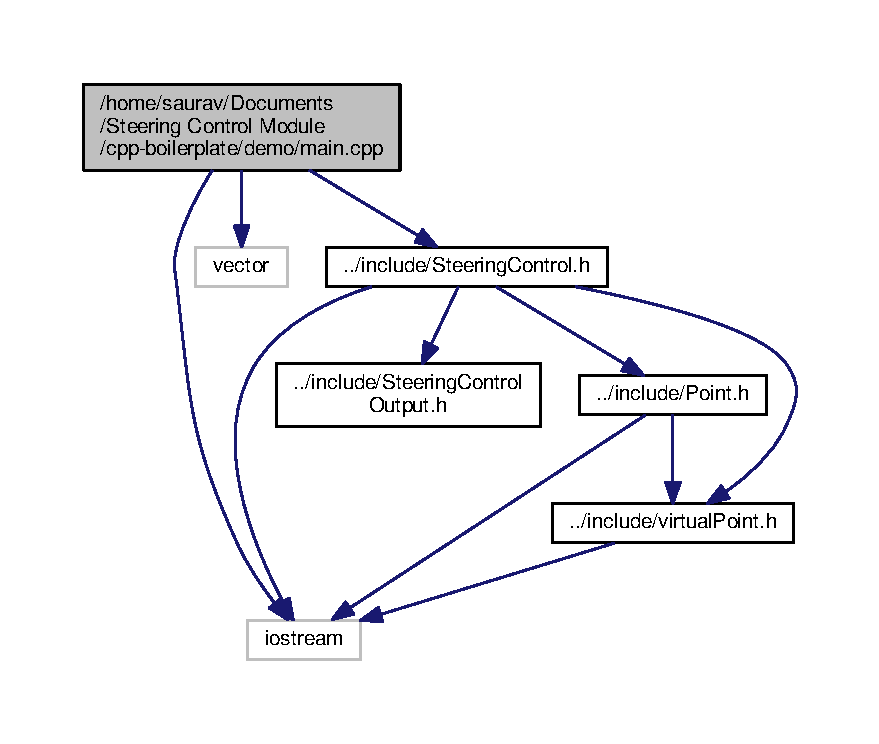
\includegraphics[width=350pt]{demo_2main_8cpp__incl}
\end{center}
\end{figure}
\subsection*{Macros}
\begin{DoxyCompactItemize}
\item 
\#define \hyperlink{demo_2main_8cpp_a598a3330b3c21701223ee0ca14316eca}{PI}~3.\+14159265
\end{DoxyCompactItemize}
\subsection*{Functions}
\begin{DoxyCompactItemize}
\item 
int \hyperlink{demo_2main_8cpp_ae66f6b31b5ad750f1fe042a706a4e3d4}{main} ()
\end{DoxyCompactItemize}


\subsection{Detailed Description}
Takes target coordinate and vehicle velocity as input and provides individual wheel speed and steering angle as output untill the vehicle has reached the defined target coordinate. It also prints the and speed of individual drive wheels,steering angle in degree and the coorinates of wheel ends . 

\begin{DoxyAuthor}{Author}
Saurav Kumar 
\end{DoxyAuthor}
\begin{DoxyCopyright}{Copyright}
2018
\end{DoxyCopyright}
B\+SD 3-\/\+Clause License

Copyright (c) 2018, Saurav Kumar All rights reserved.

Redistribution and use in source and binary forms, with or without modification, are permitted provided that the following conditions are met\+:

Redistributions of source code must retain the above copyright notice, this list of conditions and the following disclaimer.

Redistributions in binary form must reproduce the above copyright notice, this list of conditions and the following disclaimer in the documentation and/or other materials provided with the distribution.

Neither the name of the copyright holder nor the names of its contributors may be used to endorse or promote products derived from this software without specific prior written permission.

T\+H\+IS S\+O\+F\+T\+W\+A\+RE IS P\+R\+O\+V\+I\+D\+ED BY T\+HE C\+O\+P\+Y\+R\+I\+G\+HT H\+O\+L\+D\+E\+RS A\+ND C\+O\+N\+T\+R\+I\+B\+U\+T\+O\+RS \char`\"{}\+A\+S I\+S\char`\"{} A\+ND A\+NY E\+X\+P\+R\+E\+SS OR I\+M\+P\+L\+I\+ED W\+A\+R\+R\+A\+N\+T\+I\+ES, I\+N\+C\+L\+U\+D\+I\+NG, B\+UT N\+OT L\+I\+M\+I\+T\+ED TO, T\+HE I\+M\+P\+L\+I\+ED W\+A\+R\+R\+A\+N\+T\+I\+ES OF M\+E\+R\+C\+H\+A\+N\+T\+A\+B\+I\+L\+I\+TY A\+ND F\+I\+T\+N\+E\+SS F\+OR A P\+A\+R\+T\+I\+C\+U\+L\+AR P\+U\+R\+P\+O\+SE A\+RE D\+I\+S\+C\+L\+A\+I\+M\+ED. IN NO E\+V\+E\+NT S\+H\+A\+LL T\+HE C\+O\+P\+Y\+R\+I\+G\+HT H\+O\+L\+D\+ER OR C\+O\+N\+T\+R\+I\+B\+U\+T\+O\+RS BE L\+I\+A\+B\+LE F\+OR A\+NY D\+I\+R\+E\+CT, I\+N\+D\+I\+R\+E\+CT, I\+N\+C\+I\+D\+E\+N\+T\+AL, S\+P\+E\+C\+I\+AL, E\+X\+E\+M\+P\+L\+A\+RY, OR C\+O\+N\+S\+E\+Q\+U\+E\+N\+T\+I\+AL D\+A\+M\+A\+G\+ES (I\+N\+C\+L\+U\+D\+I\+NG, B\+UT N\+OT L\+I\+M\+I\+T\+ED TO, P\+R\+O\+C\+U\+R\+E\+M\+E\+NT OF S\+U\+B\+S\+T\+I\+T\+U\+TE G\+O\+O\+DS OR S\+E\+R\+V\+I\+C\+ES; L\+O\+SS OF U\+SE, D\+A\+TA, OR P\+R\+O\+F\+I\+TS; OR B\+U\+S\+I\+N\+E\+SS I\+N\+T\+E\+R\+R\+U\+P\+T\+I\+ON) H\+O\+W\+E\+V\+ER C\+A\+U\+S\+ED A\+ND ON A\+NY T\+H\+E\+O\+RY OF L\+I\+A\+B\+I\+L\+I\+TY, W\+H\+E\+T\+H\+ER IN C\+O\+N\+T\+R\+A\+CT, S\+T\+R\+I\+CT L\+I\+A\+B\+I\+L\+I\+TY, OR T\+O\+RT (I\+N\+C\+L\+U\+D\+I\+NG N\+E\+G\+L\+I\+G\+E\+N\+CE OR O\+T\+H\+E\+R\+W\+I\+SE) A\+R\+I\+S\+I\+NG IN A\+NY W\+AY O\+UT OF T\+HE U\+SE OF T\+H\+IS S\+O\+F\+T\+W\+A\+RE, E\+V\+EN IF A\+D\+V\+I\+S\+ED OF T\+HE P\+O\+S\+S\+I\+B\+I\+L\+I\+TY OF S\+U\+CH D\+A\+M\+A\+GE. 

\subsection{Macro Definition Documentation}
\index{demo/main.\+cpp@{demo/main.\+cpp}!PI@{PI}}
\index{PI@{PI}!demo/main.\+cpp@{demo/main.\+cpp}}
\subsubsection[{\texorpdfstring{PI}{PI}}]{\setlength{\rightskip}{0pt plus 5cm}\#define PI~3.\+14159265}\hypertarget{demo_2main_8cpp_a598a3330b3c21701223ee0ca14316eca}{}\label{demo_2main_8cpp_a598a3330b3c21701223ee0ca14316eca}


\subsection{Function Documentation}
\index{demo/main.\+cpp@{demo/main.\+cpp}!main@{main}}
\index{main@{main}!demo/main.\+cpp@{demo/main.\+cpp}}
\subsubsection[{\texorpdfstring{main()}{main()}}]{\setlength{\rightskip}{0pt plus 5cm}int main (
\begin{DoxyParamCaption}
{}
\end{DoxyParamCaption}
)}\hypertarget{demo_2main_8cpp_ae66f6b31b5ad750f1fe042a706a4e3d4}{}\label{demo_2main_8cpp_ae66f6b31b5ad750f1fe042a706a4e3d4}
Takes the details of the vehicle parameters such as wheelbase, trackwitdh and the height of center of gravity along with the target coordinate and the vehicle velocity

An object is called of class \hyperlink{classSteeringControl}{Steering\+Control} and its parameters are fed

Target and the vehicle velocity is set for the object Vehicle which is taken as input.

Loop is run to until the vehicle reaches within the vicinity of target coordinate
\hypertarget{test_2main_8cpp}{}\section{/home/saurav/\+Documents/\+Steering Control Module/cpp-\/boilerplate/test/main.cpp File Reference}
\label{test_2main_8cpp}\index{/home/saurav/\+Documents/\+Steering Control Module/cpp-\/boilerplate/test/main.\+cpp@{/home/saurav/\+Documents/\+Steering Control Module/cpp-\/boilerplate/test/main.\+cpp}}


Runs unit tests using google gtest framework.  


{\ttfamily \#include $<$gtest/gtest.\+h$>$}\\*
{\ttfamily \#include $<$gmock/gmock.\+h$>$}\\*
Include dependency graph for main.\+cpp\+:
\nopagebreak
\begin{figure}[H]
\begin{center}
\leavevmode
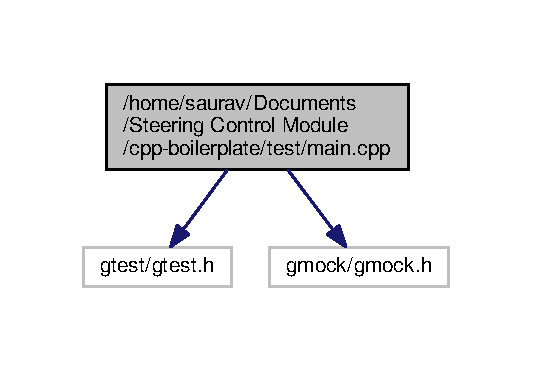
\includegraphics[width=256pt]{test_2main_8cpp__incl}
\end{center}
\end{figure}
\subsection*{Functions}
\begin{DoxyCompactItemize}
\item 
int \hyperlink{test_2main_8cpp_a3c04138a5bfe5d72780bb7e82a18e627}{main} (int argc, char $\ast$$\ast$argv)
\begin{DoxyCompactList}\small\item\em commands all tests to run \end{DoxyCompactList}\end{DoxyCompactItemize}


\subsection{Detailed Description}
Runs unit tests using google gtest framework. 

\begin{DoxyAuthor}{Author}
Saurav Kumar 
\end{DoxyAuthor}
\begin{DoxyCopyright}{Copyright}
2018
\end{DoxyCopyright}
B\+SD 3-\/\+Clause License

Copyright (c) 2018, Saurav Kumar All rights reserved.

Redistribution and use in source and binary forms, with or without modification, are permitted provided that the following conditions are met\+:

Redistributions of source code must retain the above copyright notice, this list of conditions and the following disclaimer.

Redistributions in binary form must reproduce the above copyright notice, this list of conditions and the following disclaimer in the documentation and/or other materials provided with the distribution.

Neither the name of the copyright holder nor the names of its contributors may be used to endorse or promote products derived from this software without specific prior written permission.

T\+H\+IS S\+O\+F\+T\+W\+A\+RE IS P\+R\+O\+V\+I\+D\+ED BY T\+HE C\+O\+P\+Y\+R\+I\+G\+HT H\+O\+L\+D\+E\+RS A\+ND C\+O\+N\+T\+R\+I\+B\+U\+T\+O\+RS \char`\"{}\+A\+S I\+S\char`\"{} A\+ND A\+NY E\+X\+P\+R\+E\+SS OR I\+M\+P\+L\+I\+ED W\+A\+R\+R\+A\+N\+T\+I\+ES, I\+N\+C\+L\+U\+D\+I\+NG, B\+UT N\+OT L\+I\+M\+I\+T\+ED TO, T\+HE I\+M\+P\+L\+I\+ED W\+A\+R\+R\+A\+N\+T\+I\+ES OF M\+E\+R\+C\+H\+A\+N\+T\+A\+B\+I\+L\+I\+TY A\+ND F\+I\+T\+N\+E\+SS F\+OR A P\+A\+R\+T\+I\+C\+U\+L\+AR P\+U\+R\+P\+O\+SE A\+RE D\+I\+S\+C\+L\+A\+I\+M\+ED. IN NO E\+V\+E\+NT S\+H\+A\+LL T\+HE C\+O\+P\+Y\+R\+I\+G\+HT H\+O\+L\+D\+ER OR C\+O\+N\+T\+R\+I\+B\+U\+T\+O\+RS BE L\+I\+A\+B\+LE F\+OR A\+NY D\+I\+R\+E\+CT, I\+N\+D\+I\+R\+E\+CT, I\+N\+C\+I\+D\+E\+N\+T\+AL, S\+P\+E\+C\+I\+AL, E\+X\+E\+M\+P\+L\+A\+RY, OR C\+O\+N\+S\+E\+Q\+U\+E\+N\+T\+I\+AL D\+A\+M\+A\+G\+ES (I\+N\+C\+L\+U\+D\+I\+NG, B\+UT N\+OT L\+I\+M\+I\+T\+ED TO, P\+R\+O\+C\+U\+R\+E\+M\+E\+NT OF S\+U\+B\+S\+T\+I\+T\+U\+TE G\+O\+O\+DS OR S\+E\+R\+V\+I\+C\+ES; L\+O\+SS OF U\+SE, D\+A\+TA, OR P\+R\+O\+F\+I\+TS; OR B\+U\+S\+I\+N\+E\+SS I\+N\+T\+E\+R\+R\+U\+P\+T\+I\+ON) H\+O\+W\+E\+V\+ER C\+A\+U\+S\+ED A\+ND ON A\+NY T\+H\+E\+O\+RY OF L\+I\+A\+B\+I\+L\+I\+TY, W\+H\+E\+T\+H\+ER IN C\+O\+N\+T\+R\+A\+CT, S\+T\+R\+I\+CT L\+I\+A\+B\+I\+L\+I\+TY, OR T\+O\+RT (I\+N\+C\+L\+U\+D\+I\+NG N\+E\+G\+L\+I\+G\+E\+N\+CE OR O\+T\+H\+E\+R\+W\+I\+SE) A\+R\+I\+S\+I\+NG IN A\+NY W\+AY O\+UT OF T\+HE U\+SE OF T\+H\+IS S\+O\+F\+T\+W\+A\+RE, E\+V\+EN IF A\+D\+V\+I\+S\+ED OF T\+HE P\+O\+S\+S\+I\+B\+I\+L\+I\+TY OF S\+U\+CH D\+A\+M\+A\+GE. 

\subsection{Function Documentation}
\index{test/main.\+cpp@{test/main.\+cpp}!main@{main}}
\index{main@{main}!test/main.\+cpp@{test/main.\+cpp}}
\subsubsection[{\texorpdfstring{main(int argc, char $\ast$$\ast$argv)}{main(int argc, char **argv)}}]{\setlength{\rightskip}{0pt plus 5cm}int main (
\begin{DoxyParamCaption}
\item[{int}]{argc, }
\item[{char $\ast$$\ast$}]{argv}
\end{DoxyParamCaption}
)}\hypertarget{test_2main_8cpp_a3c04138a5bfe5d72780bb7e82a18e627}{}\label{test_2main_8cpp_a3c04138a5bfe5d72780bb7e82a18e627}


commands all tests to run 


\begin{DoxyParams}{Parameters}
{\em argc} & argument count \\
\hline
{\em argv} & argument vector \\
\hline
\end{DoxyParams}
\begin{DoxyReturn}{Returns}
0 when no failures encountered 1 when failures encountered 
\end{DoxyReturn}

\hypertarget{Point_8cpp}{}\section{/home/saurav/\+Documents/\+Steering Control Module/cpp-\/boilerplate/app/\+Point.cpp File Reference}
\label{Point_8cpp}\index{/home/saurav/\+Documents/\+Steering Control Module/cpp-\/boilerplate/app/\+Point.\+cpp@{/home/saurav/\+Documents/\+Steering Control Module/cpp-\/boilerplate/app/\+Point.\+cpp}}
{\ttfamily \#include \char`\"{}../include/\+Point.\+h\char`\"{}}\\*
{\ttfamily \#include $<$math.\+h$>$}\\*
{\ttfamily \#include $<$algorithm$>$}\\*
{\ttfamily \#include $<$iostream$>$}\\*
Include dependency graph for Point.\+cpp\+:
\nopagebreak
\begin{figure}[H]
\begin{center}
\leavevmode
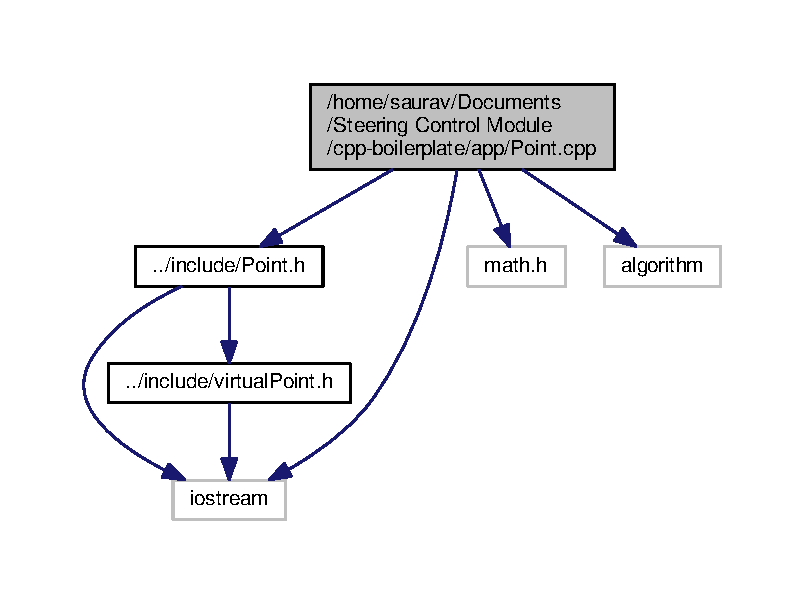
\includegraphics[width=350pt]{Point_8cpp__incl}
\end{center}
\end{figure}

\hypertarget{SteeringControl_8cpp}{}\section{/home/saurav/\+Documents/\+Steering Control Module/cpp-\/boilerplate/app/\+Steering\+Control.cpp File Reference}
\label{SteeringControl_8cpp}\index{/home/saurav/\+Documents/\+Steering Control Module/cpp-\/boilerplate/app/\+Steering\+Control.\+cpp@{/home/saurav/\+Documents/\+Steering Control Module/cpp-\/boilerplate/app/\+Steering\+Control.\+cpp}}


Takes target coordinate and vehicle velocity as input and provides individual wheel speed, steering angle, new coordinates of the vehicle wheel endafter a dt time ,such that the vehicle movement shall be toward the target point.\+The standard time latency is considered to be 0.\+01 sec.  


{\ttfamily \#include $<$math.\+h$>$}\\*
{\ttfamily \#include $<$algorithm$>$}\\*
{\ttfamily \#include $<$iostream$>$}\\*
{\ttfamily \#include \char`\"{}../include/\+Steering\+Control.\+h\char`\"{}}\\*
Include dependency graph for Steering\+Control.\+cpp\+:
\nopagebreak
\begin{figure}[H]
\begin{center}
\leavevmode
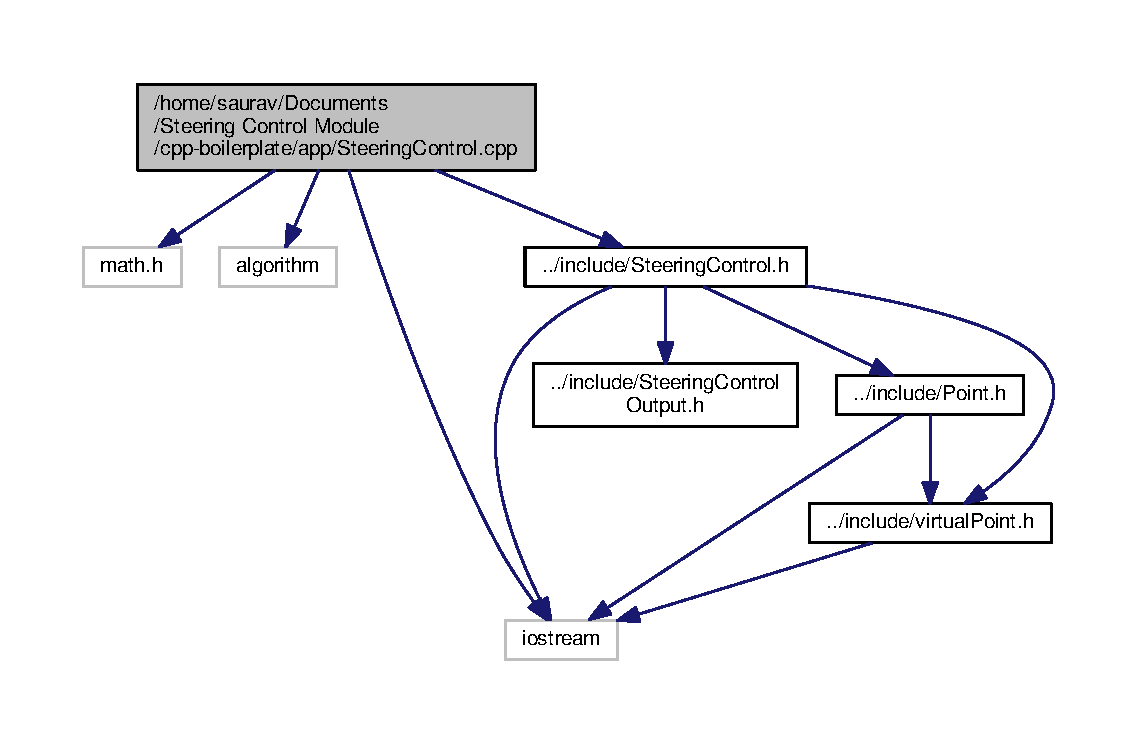
\includegraphics[width=350pt]{SteeringControl_8cpp__incl}
\end{center}
\end{figure}
\subsection*{Macros}
\begin{DoxyCompactItemize}
\item 
\#define \hyperlink{SteeringControl_8cpp_a167d2c0ec9b943d55f2124f7442b2f6d}{g}~9.\+80665
\end{DoxyCompactItemize}


\subsection{Detailed Description}
Takes target coordinate and vehicle velocity as input and provides individual wheel speed, steering angle, new coordinates of the vehicle wheel endafter a dt time ,such that the vehicle movement shall be toward the target point.\+The standard time latency is considered to be 0.\+01 sec. 

\begin{DoxyAuthor}{Author}
Saurav Kumar 
\end{DoxyAuthor}
\begin{DoxyCopyright}{Copyright}
2018
\end{DoxyCopyright}
B\+SD 3-\/\+Clause License

Copyright (c) 2018, Saurav Kumar All rights reserved.

Redistribution and use in source and binary forms, with or without modification, are permitted provided that the following conditions are met\+:

Redistributions of source code must retain the above copyright notice, this list of conditions and the following disclaimer.

Redistributions in binary form must reproduce the above copyright notice, this list of conditions and the following disclaimer in the documentation and/or other materials provided with the distribution.

Neither the name of the copyright holder nor the names of its contributors may be used to endorse or promote products derived from this software without specific prior written permission.

T\+H\+IS S\+O\+F\+T\+W\+A\+RE IS P\+R\+O\+V\+I\+D\+ED BY T\+HE C\+O\+P\+Y\+R\+I\+G\+HT H\+O\+L\+D\+E\+RS A\+ND C\+O\+N\+T\+R\+I\+B\+U\+T\+O\+RS \char`\"{}\+A\+S I\+S\char`\"{} A\+ND A\+NY E\+X\+P\+R\+E\+SS OR I\+M\+P\+L\+I\+ED W\+A\+R\+R\+A\+N\+T\+I\+ES, I\+N\+C\+L\+U\+D\+I\+NG, B\+UT N\+OT L\+I\+M\+I\+T\+ED TO, T\+HE I\+M\+P\+L\+I\+ED W\+A\+R\+R\+A\+N\+T\+I\+ES OF M\+E\+R\+C\+H\+A\+N\+T\+A\+B\+I\+L\+I\+TY A\+ND F\+I\+T\+N\+E\+SS F\+OR A P\+A\+R\+T\+I\+C\+U\+L\+AR P\+U\+R\+P\+O\+SE A\+RE D\+I\+S\+C\+L\+A\+I\+M\+ED. IN NO E\+V\+E\+NT S\+H\+A\+LL T\+HE C\+O\+P\+Y\+R\+I\+G\+HT H\+O\+L\+D\+ER OR C\+O\+N\+T\+R\+I\+B\+U\+T\+O\+RS BE L\+I\+A\+B\+LE F\+OR A\+NY D\+I\+R\+E\+CT, I\+N\+D\+I\+R\+E\+CT, I\+N\+C\+I\+D\+E\+N\+T\+AL, S\+P\+E\+C\+I\+AL, E\+X\+E\+M\+P\+L\+A\+RY, OR C\+O\+N\+S\+E\+Q\+U\+E\+N\+T\+I\+AL D\+A\+M\+A\+G\+ES (I\+N\+C\+L\+U\+D\+I\+NG, B\+UT N\+OT L\+I\+M\+I\+T\+ED TO, P\+R\+O\+C\+U\+R\+E\+M\+E\+NT OF S\+U\+B\+S\+T\+I\+T\+U\+TE G\+O\+O\+DS OR S\+E\+R\+V\+I\+C\+ES; L\+O\+SS OF U\+SE, D\+A\+TA, OR P\+R\+O\+F\+I\+TS; OR B\+U\+S\+I\+N\+E\+SS I\+N\+T\+E\+R\+R\+U\+P\+T\+I\+ON) H\+O\+W\+E\+V\+ER C\+A\+U\+S\+ED A\+ND ON A\+NY T\+H\+E\+O\+RY OF L\+I\+A\+B\+I\+L\+I\+TY, W\+H\+E\+T\+H\+ER IN C\+O\+N\+T\+R\+A\+CT, S\+T\+R\+I\+CT L\+I\+A\+B\+I\+L\+I\+TY, OR T\+O\+RT (I\+N\+C\+L\+U\+D\+I\+NG N\+E\+G\+L\+I\+G\+E\+N\+CE OR O\+T\+H\+E\+R\+W\+I\+SE) A\+R\+I\+S\+I\+NG IN A\+NY W\+AY O\+UT OF T\+HE U\+SE OF T\+H\+IS S\+O\+F\+T\+W\+A\+RE, E\+V\+EN IF A\+D\+V\+I\+S\+ED OF T\+HE P\+O\+S\+S\+I\+B\+I\+L\+I\+TY OF S\+U\+CH D\+A\+M\+A\+GE. 

\subsection{Macro Definition Documentation}
\index{Steering\+Control.\+cpp@{Steering\+Control.\+cpp}!g@{g}}
\index{g@{g}!Steering\+Control.\+cpp@{Steering\+Control.\+cpp}}
\subsubsection[{\texorpdfstring{g}{g}}]{\setlength{\rightskip}{0pt plus 5cm}\#define g~9.\+80665}\hypertarget{SteeringControl_8cpp_a167d2c0ec9b943d55f2124f7442b2f6d}{}\label{SteeringControl_8cpp_a167d2c0ec9b943d55f2124f7442b2f6d}

\hypertarget{SteeringControlOutput_8cpp}{}\section{/home/saurav/\+Documents/\+Steering Control Module/cpp-\/boilerplate/app/\+Steering\+Control\+Output.cpp File Reference}
\label{SteeringControlOutput_8cpp}\index{/home/saurav/\+Documents/\+Steering Control Module/cpp-\/boilerplate/app/\+Steering\+Control\+Output.\+cpp@{/home/saurav/\+Documents/\+Steering Control Module/cpp-\/boilerplate/app/\+Steering\+Control\+Output.\+cpp}}
{\ttfamily \#include \char`\"{}../include/\+Steering\+Control\+Output.\+h\char`\"{}}\\*
{\ttfamily \#include $<$math.\+h$>$}\\*
{\ttfamily \#include $<$algorithm$>$}\\*
{\ttfamily \#include $<$iostream$>$}\\*
Include dependency graph for Steering\+Control\+Output.\+cpp\+:
\nopagebreak
\begin{figure}[H]
\begin{center}
\leavevmode
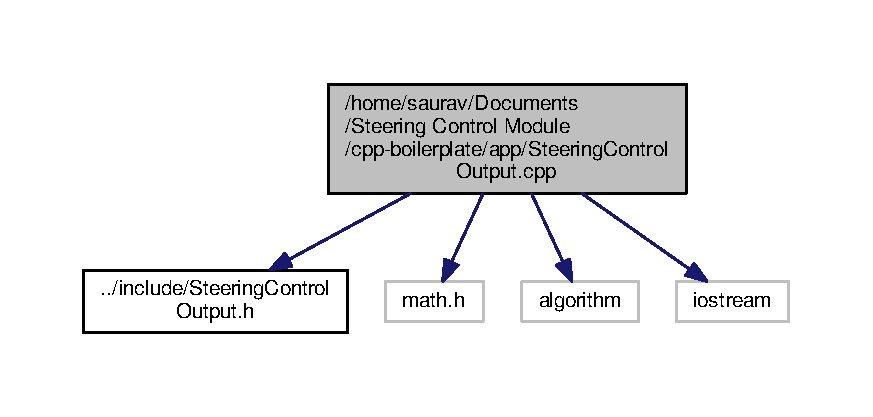
\includegraphics[width=350pt]{SteeringControlOutput_8cpp__incl}
\end{center}
\end{figure}

\hypertarget{Point_8h}{}\section{/home/saurav/\+Documents/\+Steering Control Module/cpp-\/boilerplate/include/\+Point.h File Reference}
\label{Point_8h}\index{/home/saurav/\+Documents/\+Steering Control Module/cpp-\/boilerplate/include/\+Point.\+h@{/home/saurav/\+Documents/\+Steering Control Module/cpp-\/boilerplate/include/\+Point.\+h}}
{\ttfamily \#include $<$iostream$>$}\\*
{\ttfamily \#include \char`\"{}../include/virtual\+Point.\+h\char`\"{}}\\*
Include dependency graph for Point.\+h\+:
\nopagebreak
\begin{figure}[H]
\begin{center}
\leavevmode
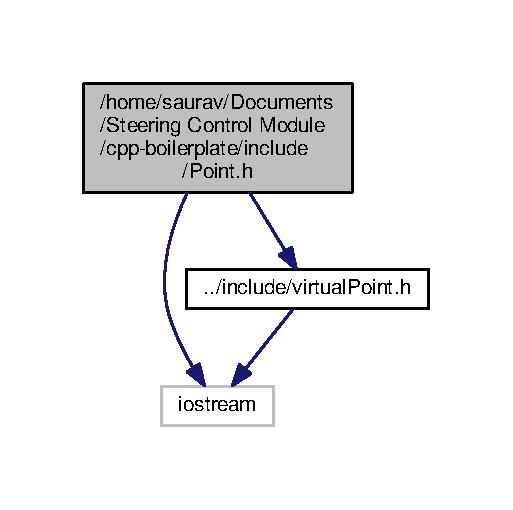
\includegraphics[width=246pt]{Point_8h__incl}
\end{center}
\end{figure}
This graph shows which files directly or indirectly include this file\+:
\nopagebreak
\begin{figure}[H]
\begin{center}
\leavevmode
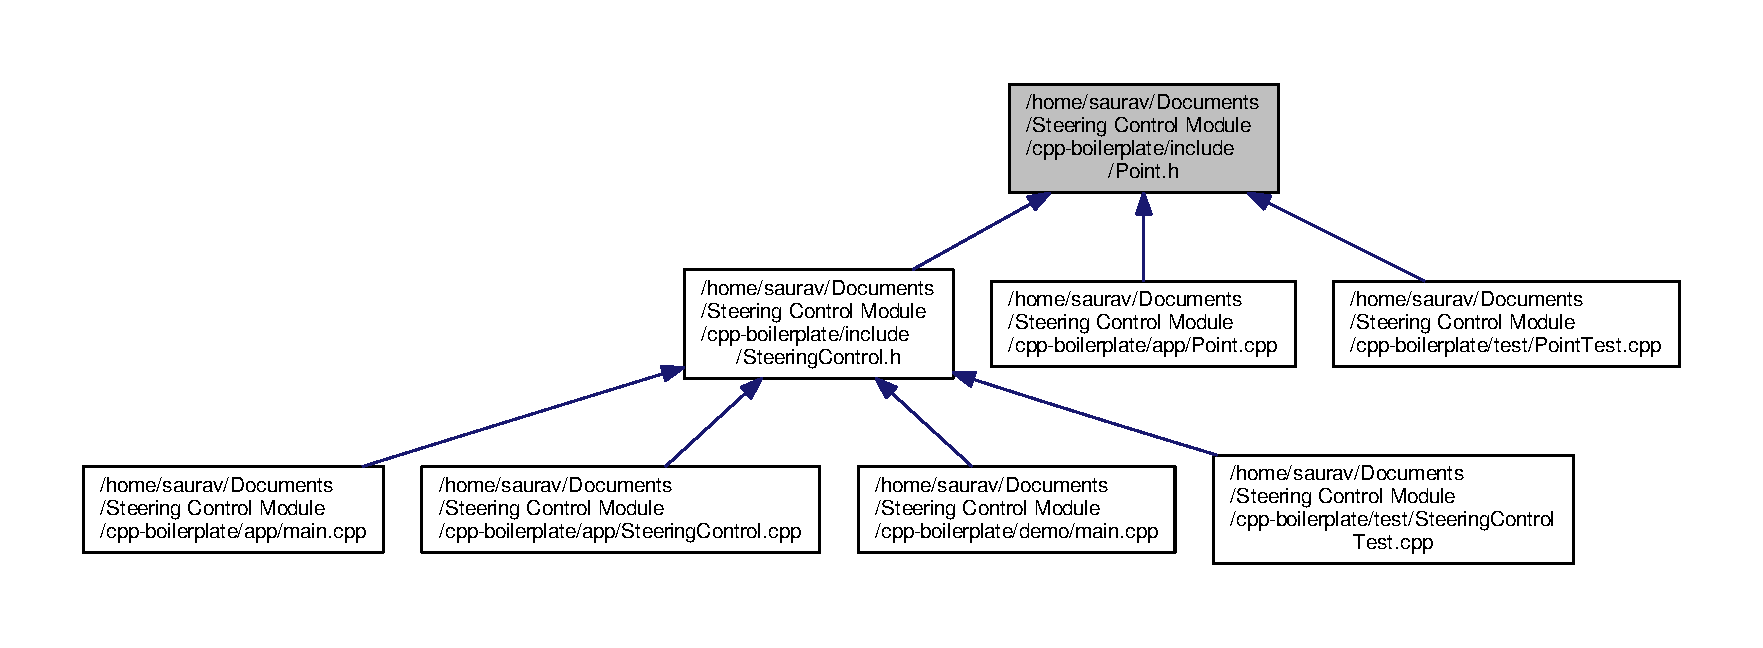
\includegraphics[width=350pt]{Point_8h__dep__incl}
\end{center}
\end{figure}
\subsection*{Classes}
\begin{DoxyCompactItemize}
\item 
class \hyperlink{classPoint}{Point}
\begin{DoxyCompactList}\small\item\em class \hyperlink{classPoint}{Point} is declared with its two data members namely X and Y and four methods \+: get\+\_\+x set\+\_\+x get\+\_\+y set\+\_\+y \end{DoxyCompactList}\end{DoxyCompactItemize}

\hypertarget{SteeringControl_8h}{}\section{/home/saurav/\+Documents/\+Steering Control Module/cpp-\/boilerplate/include/\+Steering\+Control.h File Reference}
\label{SteeringControl_8h}\index{/home/saurav/\+Documents/\+Steering Control Module/cpp-\/boilerplate/include/\+Steering\+Control.\+h@{/home/saurav/\+Documents/\+Steering Control Module/cpp-\/boilerplate/include/\+Steering\+Control.\+h}}


Header file for declaring the class \hyperlink{classSteeringControl}{Steering\+Control},its attributes and its methods along with class \hyperlink{classSteeringControlOutput}{Steering\+Control\+Output}, class \hyperlink{classPoint}{Point} and their data members.  


{\ttfamily \#include $<$iostream$>$}\\*
{\ttfamily \#include \char`\"{}../include/\+Steering\+Control\+Output.\+h\char`\"{}}\\*
{\ttfamily \#include \char`\"{}../include/\+Point.\+h\char`\"{}}\\*
{\ttfamily \#include \char`\"{}../include/virtual\+Point.\+h\char`\"{}}\\*
Include dependency graph for Steering\+Control.\+h\+:
\nopagebreak
\begin{figure}[H]
\begin{center}
\leavevmode
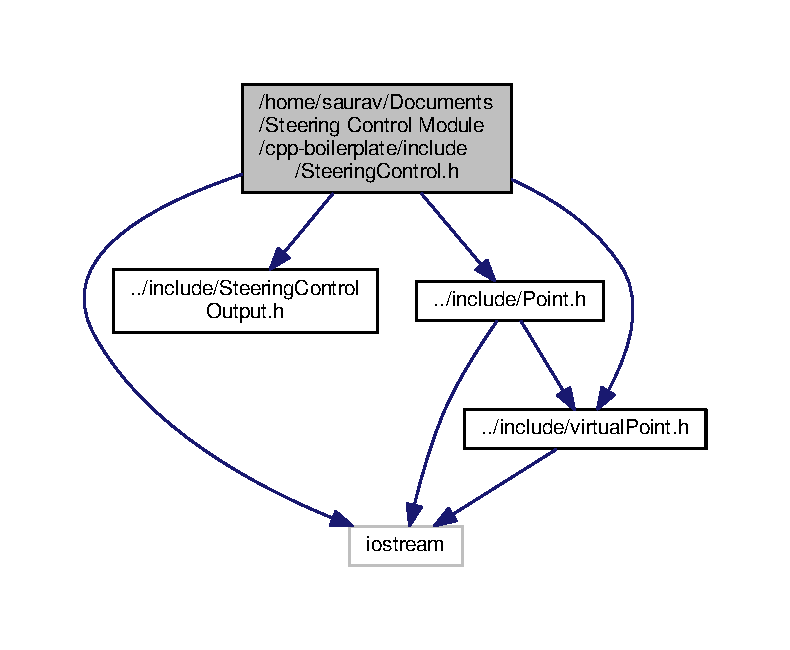
\includegraphics[width=350pt]{SteeringControl_8h__incl}
\end{center}
\end{figure}
This graph shows which files directly or indirectly include this file\+:
\nopagebreak
\begin{figure}[H]
\begin{center}
\leavevmode
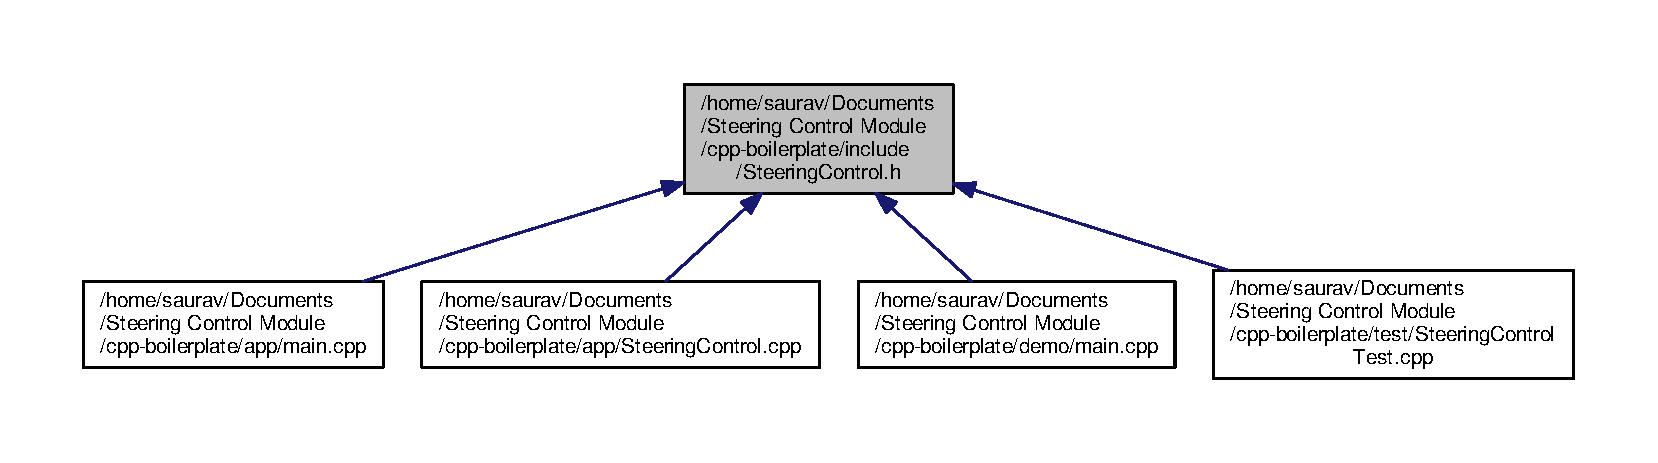
\includegraphics[width=350pt]{SteeringControl_8h__dep__incl}
\end{center}
\end{figure}
\subsection*{Classes}
\begin{DoxyCompactItemize}
\item 
class \hyperlink{classSteeringControl}{Steering\+Control}
\begin{DoxyCompactList}\small\item\em class \hyperlink{classSteeringControl}{Steering\+Control} is declared with its four double type private data members (wheelbase, trackwidth, cgz, vehicle\+Velocity) and four \hyperlink{classPoint}{Point(class)}type data members (Target, Veh\+Front, Veh\+Right, Veh\+Left) class \hyperlink{classSteeringControl}{Steering\+Control} has seven methods \+: compute\+\_\+and\+\_\+update\+\_\+coordinate set\+\_\+target\+\_\+and\+\_\+veh\+\_\+velocity get\+\_\+distance has\+\_\+reached\+\_\+target, get\+\_\+front\+\_\+coordinate, get\+\_\+left\+\_\+coordinate, get\+\_\+right\+\_\+coordinate \end{DoxyCompactList}\end{DoxyCompactItemize}


\subsection{Detailed Description}
Header file for declaring the class \hyperlink{classSteeringControl}{Steering\+Control},its attributes and its methods along with class \hyperlink{classSteeringControlOutput}{Steering\+Control\+Output}, class \hyperlink{classPoint}{Point} and their data members. 

\begin{DoxyAuthor}{Author}
Saurav Kumar 
\end{DoxyAuthor}
\begin{DoxyCopyright}{Copyright}
2018
\end{DoxyCopyright}
B\+SD 3-\/\+Clause License

Copyright (c) 2018, Saurav Kumar All rights reserved.

Redistribution and use in source and binary forms, with or without modification, are permitted provided that the following conditions are met\+:

Redistributions of source code must retain the above copyright notice, this list of conditions and the following disclaimer.

Redistributions in binary form must reproduce the above copyright notice, this list of conditions and the following disclaimer in the documentation and/or other materials provided with the distribution.

Neither the name of the copyright holder nor the names of its contributors may be used to endorse or promote products derived from this software without specific prior written permission.

T\+H\+IS S\+O\+F\+T\+W\+A\+RE IS P\+R\+O\+V\+I\+D\+ED BY T\+HE C\+O\+P\+Y\+R\+I\+G\+HT H\+O\+L\+D\+E\+RS A\+ND C\+O\+N\+T\+R\+I\+B\+U\+T\+O\+RS \char`\"{}\+A\+S I\+S\char`\"{} A\+ND A\+NY E\+X\+P\+R\+E\+SS OR I\+M\+P\+L\+I\+ED W\+A\+R\+R\+A\+N\+T\+I\+ES, I\+N\+C\+L\+U\+D\+I\+NG, B\+UT N\+OT L\+I\+M\+I\+T\+ED TO, T\+HE I\+M\+P\+L\+I\+ED W\+A\+R\+R\+A\+N\+T\+I\+ES OF M\+E\+R\+C\+H\+A\+N\+T\+A\+B\+I\+L\+I\+TY A\+ND F\+I\+T\+N\+E\+SS F\+OR A P\+A\+R\+T\+I\+C\+U\+L\+AR P\+U\+R\+P\+O\+SE A\+RE D\+I\+S\+C\+L\+A\+I\+M\+ED. IN NO E\+V\+E\+NT S\+H\+A\+LL T\+HE C\+O\+P\+Y\+R\+I\+G\+HT H\+O\+L\+D\+ER OR C\+O\+N\+T\+R\+I\+B\+U\+T\+O\+RS BE L\+I\+A\+B\+LE F\+OR A\+NY D\+I\+R\+E\+CT, I\+N\+D\+I\+R\+E\+CT, I\+N\+C\+I\+D\+E\+N\+T\+AL, S\+P\+E\+C\+I\+AL, E\+X\+E\+M\+P\+L\+A\+RY, OR C\+O\+N\+S\+E\+Q\+U\+E\+N\+T\+I\+AL D\+A\+M\+A\+G\+ES (I\+N\+C\+L\+U\+D\+I\+NG, B\+UT N\+OT L\+I\+M\+I\+T\+ED TO, P\+R\+O\+C\+U\+R\+E\+M\+E\+NT OF S\+U\+B\+S\+T\+I\+T\+U\+TE G\+O\+O\+DS OR S\+E\+R\+V\+I\+C\+ES; L\+O\+SS OF U\+SE, D\+A\+TA, OR P\+R\+O\+F\+I\+TS; OR B\+U\+S\+I\+N\+E\+SS I\+N\+T\+E\+R\+R\+U\+P\+T\+I\+ON) H\+O\+W\+E\+V\+ER C\+A\+U\+S\+ED A\+ND ON A\+NY T\+H\+E\+O\+RY OF L\+I\+A\+B\+I\+L\+I\+TY, W\+H\+E\+T\+H\+ER IN C\+O\+N\+T\+R\+A\+CT, S\+T\+R\+I\+CT L\+I\+A\+B\+I\+L\+I\+TY, OR T\+O\+RT (I\+N\+C\+L\+U\+D\+I\+NG N\+E\+G\+L\+I\+G\+E\+N\+CE OR O\+T\+H\+E\+R\+W\+I\+SE) A\+R\+I\+S\+I\+NG IN A\+NY W\+AY O\+UT OF T\+HE U\+SE OF T\+H\+IS S\+O\+F\+T\+W\+A\+RE, E\+V\+EN IF A\+D\+V\+I\+S\+ED OF T\+HE P\+O\+S\+S\+I\+B\+I\+L\+I\+TY OF S\+U\+CH D\+A\+M\+A\+GE. 
\hypertarget{SteeringControlOutput_8h}{}\section{/home/saurav/\+Documents/\+Steering Control Module/cpp-\/boilerplate/include/\+Steering\+Control\+Output.h File Reference}
\label{SteeringControlOutput_8h}\index{/home/saurav/\+Documents/\+Steering Control Module/cpp-\/boilerplate/include/\+Steering\+Control\+Output.\+h@{/home/saurav/\+Documents/\+Steering Control Module/cpp-\/boilerplate/include/\+Steering\+Control\+Output.\+h}}
This graph shows which files directly or indirectly include this file\+:
\nopagebreak
\begin{figure}[H]
\begin{center}
\leavevmode
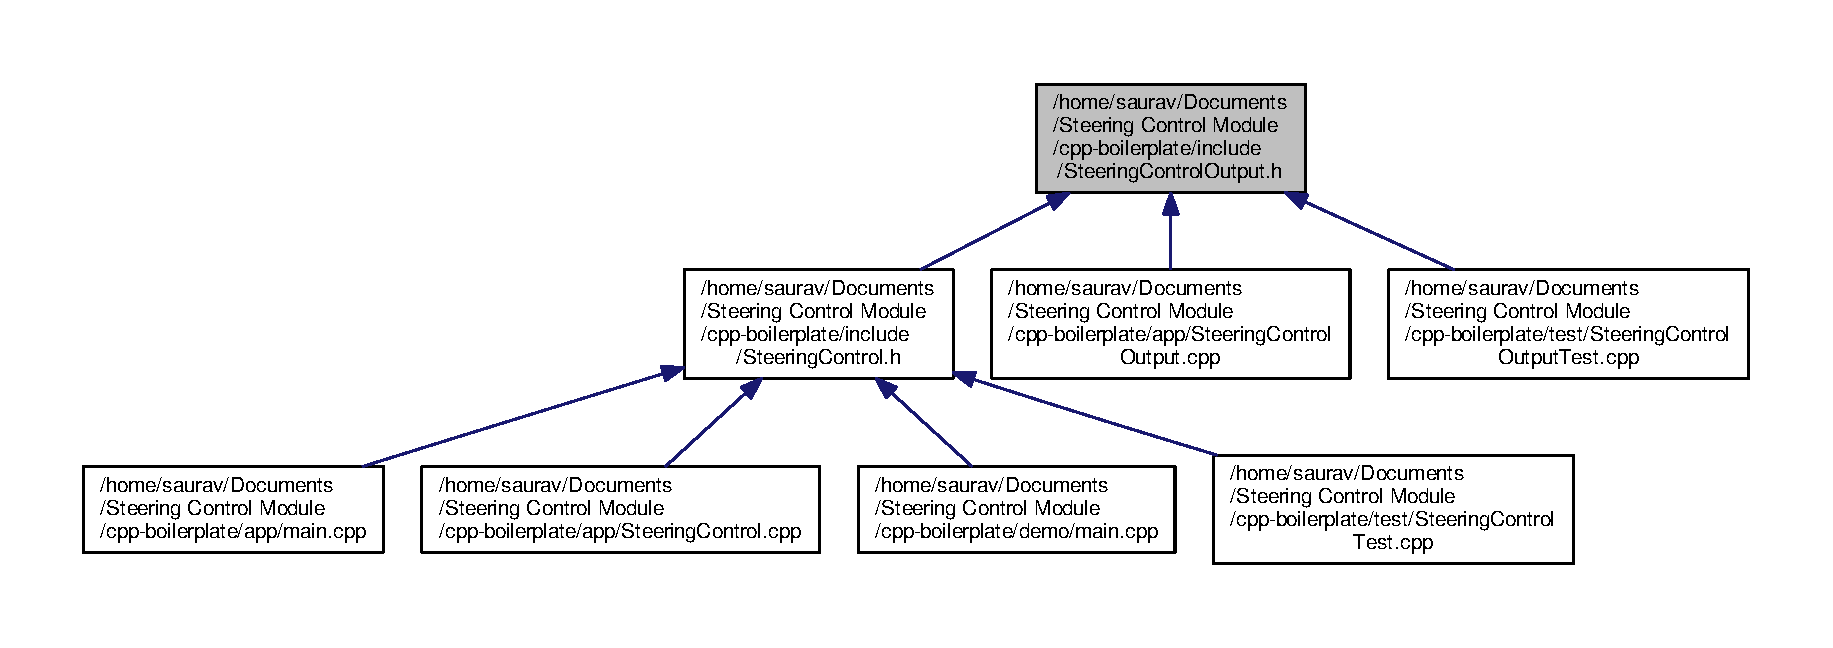
\includegraphics[width=350pt]{SteeringControlOutput_8h__dep__incl}
\end{center}
\end{figure}
\subsection*{Classes}
\begin{DoxyCompactItemize}
\item 
class \hyperlink{classSteeringControlOutput}{Steering\+Control\+Output}
\begin{DoxyCompactList}\small\item\em class \hyperlink{classSteeringControlOutput}{Steering\+Control\+Output} is declared with its three data members namely Left\+Wheel\+Speed, Right\+Wheel\+Speed and Steering\+Angle and have six methods \+: get\+\_\+left\+\_\+wheel\+\_\+speed set\+\_\+left\+\_\+wheel\+\_\+speed get\+\_\+right\+\_\+wheel\+\_\+speed set\+\_\+right\+\_\+wheel\+\_\+speed get\+\_\+steering\+\_\+angle set\+\_\+steering\+\_\+angle \end{DoxyCompactList}\end{DoxyCompactItemize}

\hypertarget{virtualPoint_8h}{}\section{/home/saurav/\+Documents/\+Steering Control Module/cpp-\/boilerplate/include/virtual\+Point.h File Reference}
\label{virtualPoint_8h}\index{/home/saurav/\+Documents/\+Steering Control Module/cpp-\/boilerplate/include/virtual\+Point.\+h@{/home/saurav/\+Documents/\+Steering Control Module/cpp-\/boilerplate/include/virtual\+Point.\+h}}
{\ttfamily \#include $<$iostream$>$}\\*
Include dependency graph for virtual\+Point.\+h\+:
\nopagebreak
\begin{figure}[H]
\begin{center}
\leavevmode
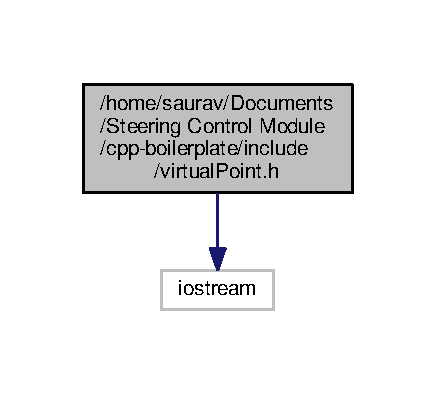
\includegraphics[width=209pt]{virtualPoint_8h__incl}
\end{center}
\end{figure}
This graph shows which files directly or indirectly include this file\+:
\nopagebreak
\begin{figure}[H]
\begin{center}
\leavevmode
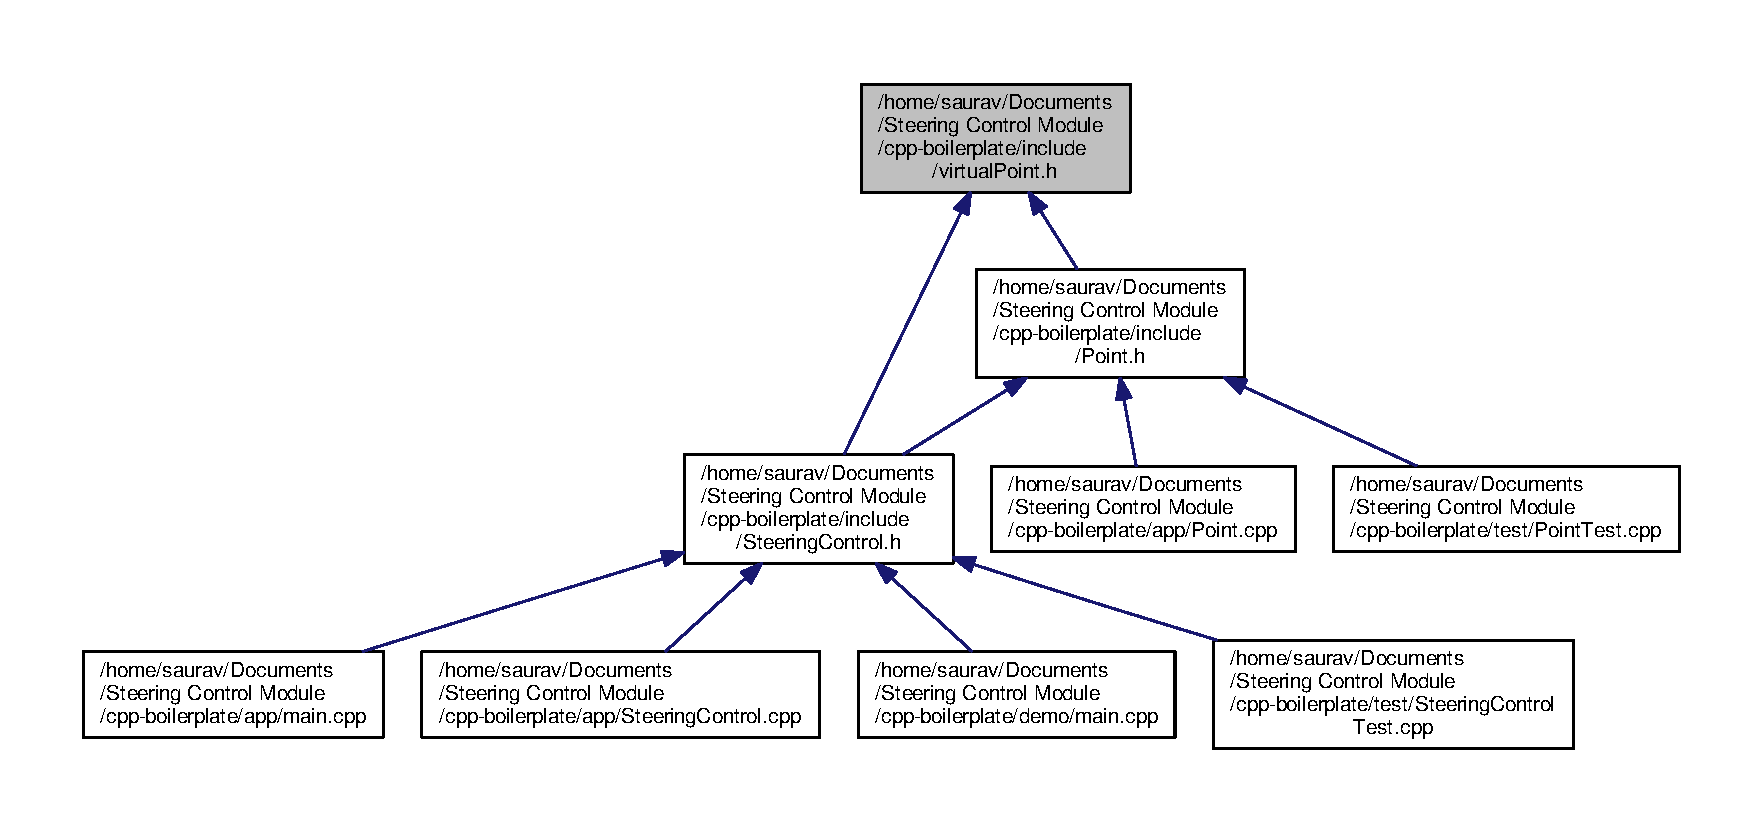
\includegraphics[width=350pt]{virtualPoint_8h__dep__incl}
\end{center}
\end{figure}
\subsection*{Classes}
\begin{DoxyCompactItemize}
\item 
class \hyperlink{classvirtualPoint}{virtual\+Point}
\end{DoxyCompactItemize}

\hypertarget{PointTest_8cpp}{}\section{/home/saurav/\+Documents/\+Steering Control Module/cpp-\/boilerplate/test/\+Point\+Test.cpp File Reference}
\label{PointTest_8cpp}\index{/home/saurav/\+Documents/\+Steering Control Module/cpp-\/boilerplate/test/\+Point\+Test.\+cpp@{/home/saurav/\+Documents/\+Steering Control Module/cpp-\/boilerplate/test/\+Point\+Test.\+cpp}}
{\ttfamily \#include $<$gtest/gtest.\+h$>$}\\*
{\ttfamily \#include \char`\"{}../include/\+Point.\+h\char`\"{}}\\*
Include dependency graph for Point\+Test.\+cpp\+:
\nopagebreak
\begin{figure}[H]
\begin{center}
\leavevmode
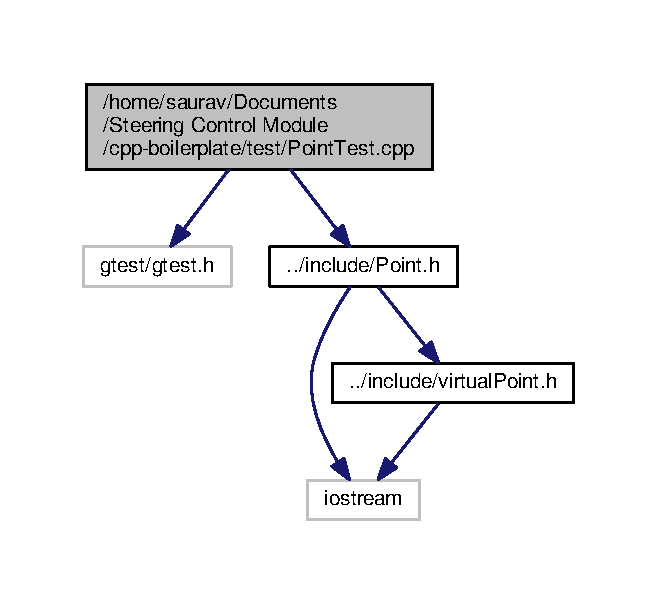
\includegraphics[width=316pt]{PointTest_8cpp__incl}
\end{center}
\end{figure}
\subsection*{Functions}
\begin{DoxyCompactItemize}
\item 
\hyperlink{PointTest_8cpp_a63688f3d43c46b5b5a8c306d99b8f872}{T\+E\+ST} (Point\+Test, get\+\_\+x\+Test)
\item 
\hyperlink{PointTest_8cpp_a4ea368b56873987418b76bb465961c0b}{T\+E\+ST} (Point\+Test, get\+\_\+y\+Test)
\begin{DoxyCompactList}\small\item\em Tests get\+\_\+front\+\_\+coordinate method. \end{DoxyCompactList}\end{DoxyCompactItemize}


\subsection{Function Documentation}
\index{Point\+Test.\+cpp@{Point\+Test.\+cpp}!T\+E\+ST@{T\+E\+ST}}
\index{T\+E\+ST@{T\+E\+ST}!Point\+Test.\+cpp@{Point\+Test.\+cpp}}
\subsubsection[{\texorpdfstring{T\+E\+S\+T(\+Point\+Test, get\+\_\+x\+Test)}{TEST(PointTest, get_xTest)}}]{\setlength{\rightskip}{0pt plus 5cm}T\+E\+ST (
\begin{DoxyParamCaption}
\item[{Point\+Test}]{, }
\item[{get\+\_\+x\+Test}]{}
\end{DoxyParamCaption}
)}\hypertarget{PointTest_8cpp_a63688f3d43c46b5b5a8c306d99b8f872}{}\label{PointTest_8cpp_a63688f3d43c46b5b5a8c306d99b8f872}
\index{Point\+Test.\+cpp@{Point\+Test.\+cpp}!T\+E\+ST@{T\+E\+ST}}
\index{T\+E\+ST@{T\+E\+ST}!Point\+Test.\+cpp@{Point\+Test.\+cpp}}
\subsubsection[{\texorpdfstring{T\+E\+S\+T(\+Point\+Test, get\+\_\+y\+Test)}{TEST(PointTest, get_yTest)}}]{\setlength{\rightskip}{0pt plus 5cm}T\+E\+ST (
\begin{DoxyParamCaption}
\item[{Point\+Test}]{, }
\item[{get\+\_\+y\+Test}]{}
\end{DoxyParamCaption}
)}\hypertarget{PointTest_8cpp_a4ea368b56873987418b76bb465961c0b}{}\label{PointTest_8cpp_a4ea368b56873987418b76bb465961c0b}


Tests get\+\_\+front\+\_\+coordinate method. 

Tests get\+\_\+left\+\_\+coordinate method 
\hypertarget{SteeringControlOutputTest_8cpp}{}\section{/home/saurav/\+Documents/\+Steering Control Module/cpp-\/boilerplate/test/\+Steering\+Control\+Output\+Test.cpp File Reference}
\label{SteeringControlOutputTest_8cpp}\index{/home/saurav/\+Documents/\+Steering Control Module/cpp-\/boilerplate/test/\+Steering\+Control\+Output\+Test.\+cpp@{/home/saurav/\+Documents/\+Steering Control Module/cpp-\/boilerplate/test/\+Steering\+Control\+Output\+Test.\+cpp}}
{\ttfamily \#include $<$gtest/gtest.\+h$>$}\\*
{\ttfamily \#include \char`\"{}../include/\+Steering\+Control\+Output.\+h\char`\"{}}\\*
Include dependency graph for Steering\+Control\+Output\+Test.\+cpp\+:
\nopagebreak
\begin{figure}[H]
\begin{center}
\leavevmode
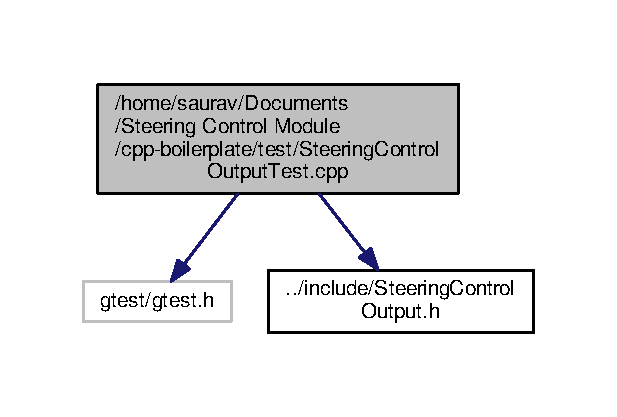
\includegraphics[width=296pt]{SteeringControlOutputTest_8cpp__incl}
\end{center}
\end{figure}
\subsection*{Functions}
\begin{DoxyCompactItemize}
\item 
\hyperlink{SteeringControlOutputTest_8cpp_ae885801dda269f429c518eb937885dea}{T\+E\+ST} (Steering\+Control\+Output\+Test, get\+\_\+left\+\_\+wheel\+\_\+speed\+Test)
\begin{DoxyCompactList}\small\item\em Tests compute\+\_\+and\+\_\+update\+\_\+coordinate method. \end{DoxyCompactList}\item 
\hyperlink{SteeringControlOutputTest_8cpp_aa447fb7c651c3a6137af917f779ecfe2}{T\+E\+ST} (Steering\+Control\+Output\+Test, get\+\_\+right\+\_\+wheel\+\_\+speedest)
\begin{DoxyCompactList}\small\item\em Tests get\+\_\+front\+\_\+coordinate method. \end{DoxyCompactList}\item 
\hyperlink{SteeringControlOutputTest_8cpp_a01112af2b7d350c02d20c4da9895e5fd}{T\+E\+ST} (Steering\+Control\+Output\+Test, get\+\_\+steering\+\_\+angle\+Test)
\end{DoxyCompactItemize}


\subsection{Function Documentation}
\index{Steering\+Control\+Output\+Test.\+cpp@{Steering\+Control\+Output\+Test.\+cpp}!T\+E\+ST@{T\+E\+ST}}
\index{T\+E\+ST@{T\+E\+ST}!Steering\+Control\+Output\+Test.\+cpp@{Steering\+Control\+Output\+Test.\+cpp}}
\subsubsection[{\texorpdfstring{T\+E\+S\+T(\+Steering\+Control\+Output\+Test, get\+\_\+left\+\_\+wheel\+\_\+speed\+Test)}{TEST(SteeringControlOutputTest, get_left_wheel_speedTest)}}]{\setlength{\rightskip}{0pt plus 5cm}T\+E\+ST (
\begin{DoxyParamCaption}
\item[{Steering\+Control\+Output\+Test}]{, }
\item[{get\+\_\+left\+\_\+wheel\+\_\+speed\+Test}]{}
\end{DoxyParamCaption}
)}\hypertarget{SteeringControlOutputTest_8cpp_ae885801dda269f429c518eb937885dea}{}\label{SteeringControlOutputTest_8cpp_ae885801dda269f429c518eb937885dea}


Tests compute\+\_\+and\+\_\+update\+\_\+coordinate method. 

\index{Steering\+Control\+Output\+Test.\+cpp@{Steering\+Control\+Output\+Test.\+cpp}!T\+E\+ST@{T\+E\+ST}}
\index{T\+E\+ST@{T\+E\+ST}!Steering\+Control\+Output\+Test.\+cpp@{Steering\+Control\+Output\+Test.\+cpp}}
\subsubsection[{\texorpdfstring{T\+E\+S\+T(\+Steering\+Control\+Output\+Test, get\+\_\+right\+\_\+wheel\+\_\+speedest)}{TEST(SteeringControlOutputTest, get_right_wheel_speedest)}}]{\setlength{\rightskip}{0pt plus 5cm}T\+E\+ST (
\begin{DoxyParamCaption}
\item[{Steering\+Control\+Output\+Test}]{, }
\item[{get\+\_\+right\+\_\+wheel\+\_\+speedest}]{}
\end{DoxyParamCaption}
)}\hypertarget{SteeringControlOutputTest_8cpp_aa447fb7c651c3a6137af917f779ecfe2}{}\label{SteeringControlOutputTest_8cpp_aa447fb7c651c3a6137af917f779ecfe2}


Tests get\+\_\+front\+\_\+coordinate method. 

\index{Steering\+Control\+Output\+Test.\+cpp@{Steering\+Control\+Output\+Test.\+cpp}!T\+E\+ST@{T\+E\+ST}}
\index{T\+E\+ST@{T\+E\+ST}!Steering\+Control\+Output\+Test.\+cpp@{Steering\+Control\+Output\+Test.\+cpp}}
\subsubsection[{\texorpdfstring{T\+E\+S\+T(\+Steering\+Control\+Output\+Test, get\+\_\+steering\+\_\+angle\+Test)}{TEST(SteeringControlOutputTest, get_steering_angleTest)}}]{\setlength{\rightskip}{0pt plus 5cm}T\+E\+ST (
\begin{DoxyParamCaption}
\item[{Steering\+Control\+Output\+Test}]{, }
\item[{get\+\_\+steering\+\_\+angle\+Test}]{}
\end{DoxyParamCaption}
)}\hypertarget{SteeringControlOutputTest_8cpp_a01112af2b7d350c02d20c4da9895e5fd}{}\label{SteeringControlOutputTest_8cpp_a01112af2b7d350c02d20c4da9895e5fd}

\hypertarget{SteeringControlTest_8cpp}{}\section{/home/saurav/\+Documents/\+Steering Control Module/cpp-\/boilerplate/test/\+Steering\+Control\+Test.cpp File Reference}
\label{SteeringControlTest_8cpp}\index{/home/saurav/\+Documents/\+Steering Control Module/cpp-\/boilerplate/test/\+Steering\+Control\+Test.\+cpp@{/home/saurav/\+Documents/\+Steering Control Module/cpp-\/boilerplate/test/\+Steering\+Control\+Test.\+cpp}}
{\ttfamily \#include $<$gtest/gtest.\+h$>$}\\*
{\ttfamily \#include $<$gmock/gmock.\+h$>$}\\*
{\ttfamily \#include \char`\"{}../include/\+Steering\+Control.\+h\char`\"{}}\\*
Include dependency graph for Steering\+Control\+Test.\+cpp\+:
\nopagebreak
\begin{figure}[H]
\begin{center}
\leavevmode
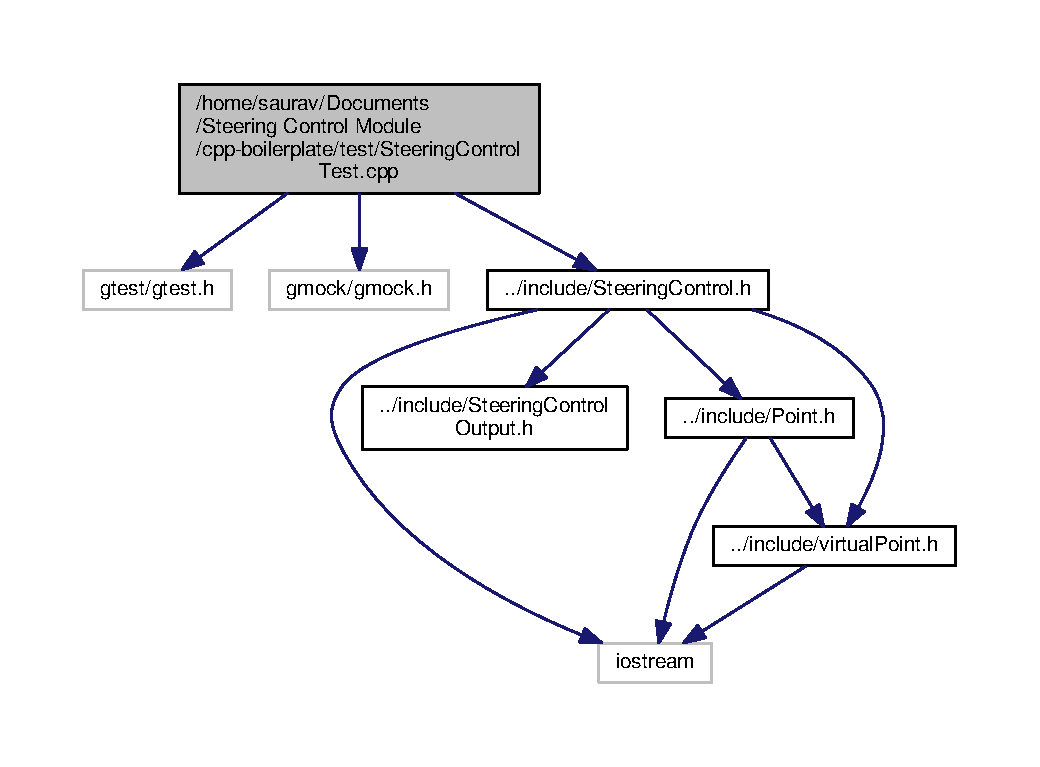
\includegraphics[width=350pt]{SteeringControlTest_8cpp__incl}
\end{center}
\end{figure}
\subsection*{Classes}
\begin{DoxyCompactItemize}
\item 
class \hyperlink{classMockPoint}{Mock\+Point}
\end{DoxyCompactItemize}
\subsection*{Functions}
\begin{DoxyCompactItemize}
\item 
\hyperlink{SteeringControlTest_8cpp_aa390e32399d73a892b54b69b22ccf93f}{T\+E\+ST} (Steering\+Control\+Test, compute\+\_\+and\+\_\+update\+\_\+coordinate\+Test)
\begin{DoxyCompactList}\small\item\em Tests compute\+\_\+and\+\_\+update\+\_\+coordinate method. \end{DoxyCompactList}\item 
\hyperlink{SteeringControlTest_8cpp_a686b0dc0ce50bd5414695390046ac81e}{T\+E\+ST} (Steering\+Control\+Test, get\+\_\+front\+\_\+coordinate\+Test)
\begin{DoxyCompactList}\small\item\em Tests get\+\_\+front\+\_\+coordinate method. \end{DoxyCompactList}\item 
\hyperlink{SteeringControlTest_8cpp_a7ce1808820d2f9c01e78040da473a1c3}{T\+E\+ST} (Steering\+Control\+Test, get\+\_\+left\+\_\+coordinate\+Test)
\begin{DoxyCompactList}\small\item\em Tests get\+\_\+left\+\_\+coordinate method. \end{DoxyCompactList}\item 
\hyperlink{SteeringControlTest_8cpp_ac3656d60d08dfc5373ac2af0a0d4e321}{T\+E\+ST} (Steering\+Control\+Test, get\+\_\+right\+\_\+coordinate\+Test)
\begin{DoxyCompactList}\small\item\em Tests get\+\_\+right\+\_\+coordinate method. \end{DoxyCompactList}\item 
\hyperlink{SteeringControlTest_8cpp_a565ba412e725071d8821355aceb0e7bf}{T\+E\+ST} (Steering\+Control\+Test, set\+\_\+vehicle\+\_\+dimension\+Test)
\begin{DoxyCompactList}\small\item\em Tests set\+\_\+vehicle\+\_\+dimension method. \end{DoxyCompactList}\item 
\hyperlink{SteeringControlTest_8cpp_a5162ace8c7a7eca7f1bb7442609a1b5f}{T\+E\+ST} (Steering\+Control\+Test, has\+\_\+reached\+\_\+target\+Test)
\begin{DoxyCompactList}\small\item\em has\+\_\+reached\+\_\+target method \end{DoxyCompactList}\item 
\hyperlink{SteeringControlTest_8cpp_ae2c8003a6c7739817eb621db7b4aaef4}{T\+E\+ST} (Steering\+Control\+Test, get\+\_\+distance\+Test)
\begin{DoxyCompactList}\small\item\em get\+\_\+distance method \end{DoxyCompactList}\end{DoxyCompactItemize}


\subsection{Function Documentation}
\index{Steering\+Control\+Test.\+cpp@{Steering\+Control\+Test.\+cpp}!T\+E\+ST@{T\+E\+ST}}
\index{T\+E\+ST@{T\+E\+ST}!Steering\+Control\+Test.\+cpp@{Steering\+Control\+Test.\+cpp}}
\subsubsection[{\texorpdfstring{T\+E\+S\+T(\+Steering\+Control\+Test, compute\+\_\+and\+\_\+update\+\_\+coordinate\+Test)}{TEST(SteeringControlTest, compute_and_update_coordinateTest)}}]{\setlength{\rightskip}{0pt plus 5cm}T\+E\+ST (
\begin{DoxyParamCaption}
\item[{Steering\+Control\+Test}]{, }
\item[{compute\+\_\+and\+\_\+update\+\_\+coordinate\+Test}]{}
\end{DoxyParamCaption}
)}\hypertarget{SteeringControlTest_8cpp_aa390e32399d73a892b54b69b22ccf93f}{}\label{SteeringControlTest_8cpp_aa390e32399d73a892b54b69b22ccf93f}


Tests compute\+\_\+and\+\_\+update\+\_\+coordinate method. 

\index{Steering\+Control\+Test.\+cpp@{Steering\+Control\+Test.\+cpp}!T\+E\+ST@{T\+E\+ST}}
\index{T\+E\+ST@{T\+E\+ST}!Steering\+Control\+Test.\+cpp@{Steering\+Control\+Test.\+cpp}}
\subsubsection[{\texorpdfstring{T\+E\+S\+T(\+Steering\+Control\+Test, get\+\_\+front\+\_\+coordinate\+Test)}{TEST(SteeringControlTest, get_front_coordinateTest)}}]{\setlength{\rightskip}{0pt plus 5cm}T\+E\+ST (
\begin{DoxyParamCaption}
\item[{Steering\+Control\+Test}]{, }
\item[{get\+\_\+front\+\_\+coordinate\+Test}]{}
\end{DoxyParamCaption}
)}\hypertarget{SteeringControlTest_8cpp_a686b0dc0ce50bd5414695390046ac81e}{}\label{SteeringControlTest_8cpp_a686b0dc0ce50bd5414695390046ac81e}


Tests get\+\_\+front\+\_\+coordinate method. 

\index{Steering\+Control\+Test.\+cpp@{Steering\+Control\+Test.\+cpp}!T\+E\+ST@{T\+E\+ST}}
\index{T\+E\+ST@{T\+E\+ST}!Steering\+Control\+Test.\+cpp@{Steering\+Control\+Test.\+cpp}}
\subsubsection[{\texorpdfstring{T\+E\+S\+T(\+Steering\+Control\+Test, get\+\_\+left\+\_\+coordinate\+Test)}{TEST(SteeringControlTest, get_left_coordinateTest)}}]{\setlength{\rightskip}{0pt plus 5cm}T\+E\+ST (
\begin{DoxyParamCaption}
\item[{Steering\+Control\+Test}]{, }
\item[{get\+\_\+left\+\_\+coordinate\+Test}]{}
\end{DoxyParamCaption}
)}\hypertarget{SteeringControlTest_8cpp_a7ce1808820d2f9c01e78040da473a1c3}{}\label{SteeringControlTest_8cpp_a7ce1808820d2f9c01e78040da473a1c3}


Tests get\+\_\+left\+\_\+coordinate method. 

\index{Steering\+Control\+Test.\+cpp@{Steering\+Control\+Test.\+cpp}!T\+E\+ST@{T\+E\+ST}}
\index{T\+E\+ST@{T\+E\+ST}!Steering\+Control\+Test.\+cpp@{Steering\+Control\+Test.\+cpp}}
\subsubsection[{\texorpdfstring{T\+E\+S\+T(\+Steering\+Control\+Test, get\+\_\+right\+\_\+coordinate\+Test)}{TEST(SteeringControlTest, get_right_coordinateTest)}}]{\setlength{\rightskip}{0pt plus 5cm}T\+E\+ST (
\begin{DoxyParamCaption}
\item[{Steering\+Control\+Test}]{, }
\item[{get\+\_\+right\+\_\+coordinate\+Test}]{}
\end{DoxyParamCaption}
)}\hypertarget{SteeringControlTest_8cpp_ac3656d60d08dfc5373ac2af0a0d4e321}{}\label{SteeringControlTest_8cpp_ac3656d60d08dfc5373ac2af0a0d4e321}


Tests get\+\_\+right\+\_\+coordinate method. 

\index{Steering\+Control\+Test.\+cpp@{Steering\+Control\+Test.\+cpp}!T\+E\+ST@{T\+E\+ST}}
\index{T\+E\+ST@{T\+E\+ST}!Steering\+Control\+Test.\+cpp@{Steering\+Control\+Test.\+cpp}}
\subsubsection[{\texorpdfstring{T\+E\+S\+T(\+Steering\+Control\+Test, set\+\_\+vehicle\+\_\+dimension\+Test)}{TEST(SteeringControlTest, set_vehicle_dimensionTest)}}]{\setlength{\rightskip}{0pt plus 5cm}T\+E\+ST (
\begin{DoxyParamCaption}
\item[{Steering\+Control\+Test}]{, }
\item[{set\+\_\+vehicle\+\_\+dimension\+Test}]{}
\end{DoxyParamCaption}
)}\hypertarget{SteeringControlTest_8cpp_a565ba412e725071d8821355aceb0e7bf}{}\label{SteeringControlTest_8cpp_a565ba412e725071d8821355aceb0e7bf}


Tests set\+\_\+vehicle\+\_\+dimension method. 

\index{Steering\+Control\+Test.\+cpp@{Steering\+Control\+Test.\+cpp}!T\+E\+ST@{T\+E\+ST}}
\index{T\+E\+ST@{T\+E\+ST}!Steering\+Control\+Test.\+cpp@{Steering\+Control\+Test.\+cpp}}
\subsubsection[{\texorpdfstring{T\+E\+S\+T(\+Steering\+Control\+Test, has\+\_\+reached\+\_\+target\+Test)}{TEST(SteeringControlTest, has_reached_targetTest)}}]{\setlength{\rightskip}{0pt plus 5cm}T\+E\+ST (
\begin{DoxyParamCaption}
\item[{Steering\+Control\+Test}]{, }
\item[{has\+\_\+reached\+\_\+target\+Test}]{}
\end{DoxyParamCaption}
)}\hypertarget{SteeringControlTest_8cpp_a5162ace8c7a7eca7f1bb7442609a1b5f}{}\label{SteeringControlTest_8cpp_a5162ace8c7a7eca7f1bb7442609a1b5f}


has\+\_\+reached\+\_\+target method 

\index{Steering\+Control\+Test.\+cpp@{Steering\+Control\+Test.\+cpp}!T\+E\+ST@{T\+E\+ST}}
\index{T\+E\+ST@{T\+E\+ST}!Steering\+Control\+Test.\+cpp@{Steering\+Control\+Test.\+cpp}}
\subsubsection[{\texorpdfstring{T\+E\+S\+T(\+Steering\+Control\+Test, get\+\_\+distance\+Test)}{TEST(SteeringControlTest, get_distanceTest)}}]{\setlength{\rightskip}{0pt plus 5cm}T\+E\+ST (
\begin{DoxyParamCaption}
\item[{Steering\+Control\+Test}]{, }
\item[{get\+\_\+distance\+Test}]{}
\end{DoxyParamCaption}
)}\hypertarget{SteeringControlTest_8cpp_ae2c8003a6c7739817eb621db7b4aaef4}{}\label{SteeringControlTest_8cpp_ae2c8003a6c7739817eb621db7b4aaef4}


get\+\_\+distance method 


%--- End generated contents ---

% Index
\backmatter
\newpage
\phantomsection
\clearemptydoublepage
\addcontentsline{toc}{chapter}{Index}
\printindex

\end{document}
